\documentclass{entcs}
\usepackage{CSC8498macro}

\makeatletter

\def\lastname{CSC8498}

% http://tex.stackexchange.com/questions/283141/latex-error-command-cauthor-already-defined
\makeatletter
\let\c@author\relax
\makeatother

\usepackage[backend=bibtex]{biblatex}
\addbibresource{CSC8498_Dissertation_DanNixon.bib}

\ifx\pdftexversion\undefined
\usepackage[dvips]{graphicx}
\else
\usepackage[pdftex]{graphicx}
\DeclareGraphicsRule{*}{mps}{*}{}
\fi

\usepackage{dirtree}
\usepackage{tikz}
\usetikzlibrary{shapes.geometric, arrows, positioning}
\usepackage{subcaption}

\tikzstyle{startstop} = [
  rectangle,
  rounded corners,
  minimum width=0.5cm,
  minimum height=0.6cm,
  text centered,
  draw=black,
  fill=red!30,
  font=\small
]

\tikzstyle{io} = [
  trapezium,
  trapezium left angle=70,
  trapezium right angle=110,
  minimum width=0.5cm,
  minimum height=0.5cm,
  text centered,
  draw=black,
  fill=blue!30,
  font=\small
]

\tikzstyle{process} = [
  rectangle,
  minimum width=0.5cm,
  minimum height=0.6cm,
  text centered,
  draw=black,
  fill=orange!30,
  font=\small
]

\tikzstyle{decision} = [
  diamond,
  minimum width=0.5cm,
  minimum height=0.6cm,
  text centered,
  draw=black,
  fill=green!30,
  aspect=4.5,
  font=\small
]

\tikzstyle{arrow} = [thick, ->, >=stealth, font=\small]

\pgfdeclarelayer{background}
\pgfdeclarelayer{foreground}
\pgfsetlayers{background,main,foreground}

\newcommand{\bitrect}[2]{
  \begin{pgfonlayer}{foreground}
    \draw [thick] (0,0) rectangle (#1,1);
    \pgfmathsetmacro\result{#1-1}
    \foreach \x in {1,...,\result}
      \draw [thick] (\x,1) -- (\x, 0.8);
    \end{pgfonlayer}
  \bitlabels{#1}{#2}
}

\newcommand{\rwbits}[3]{
  \draw [thick] (#1,0) rectangle ++(#2,1) node[pos=0.5]{#3};
  \pgfmathsetmacro\start{#1+0.5}
  \pgfmathsetmacro\finish{#1+#2-0.5}
}

\newcommand{\robits}[3]{
  \begin{pgfonlayer}{background}
    \draw [thick, fill=lightgray] (#1,0)
    rectangle ++(#2,1) node[pos=0.5]{#3};
  \end{pgfonlayer}
  \pgfmathsetmacro\start{#1+0.5}
  \pgfmathsetmacro\finish{#1+#2-0.5}
}

\newcommand{\bitlabels}[2] {
  \foreach \bit in {1,...,#1} {
    \pgfmathsetmacro\result{#2}
    \node [above] at (\bit-0.5, 1) {\pgfmathprintnumber{\result}};
  }
}

\begin{document}

\begin{frontmatter}
  \title{IMU informed point cloud registration}
  \author{Dan Nixon}
  \address{School of Computing Science, Newcastle University, UK}
  \thanks[email]{Email:
    \href{mailto:d.nixon2@ncl.ac.uk}
  {\texttt{\normalshape{d.nixon2@ncl.ac.uk}}}}

  \begin{abstract}
    The registration of multiple 3D point clouds is a key stage in a 3D
    scanning/environment capture workflow. The traditional method used to
    perform this task uses inspection of the 3D data to form an estimate of the
    transformation between pairs of point clouds. This report describes an
    alternative initial transform estimation method using data obtained from an
    IMU measuring the camera position and orientation. While this method
    provides a reasonable initial estimate its performance would still be
    exceeded by a properly configured feature based estimation.
  \end{abstract}

  \begin{keyword}
    3D scanning, point clouds, IMU, RGB-D
  \end{keyword}
\end{frontmatter}

\section{Introduction}

3D scanning has seen a significant increase in use over the last decade,
primarily due to the wide availability of commodity level equipment and its
ability to produce scans of a usable quality, whether that be for use in a
visualisation/simulation or manufacturing.

The increasing popularity and availability of commodity RGB-D sensors is making
them a go-to choice for short range object and environment scanning.

Given they have a finite field of view processing steps are required to convert
the captured data into a point cloud or mesh that accurately represents the
geometry being scanned.

The nature of 3D point clouds presents several methods of performing
registration of one or more point clouds. Typically starting by obtaining an
estimation of the spatial transformation between two point clouds and then
refining this transformation with a finer grained optimisation routine.

The quality of the initial transformation estimation can depend a great deal on
the shape of geometry being scanned, the scale of the environment and quality of
captured point clouds. This can make it potentially difficult to create a system
that will work reliably in multiple environments over a wide scale range.

\subsection{Background}

One of the most common and easily available RGB-D cameras is the Microsoft
Kinect. This combines a standard RGB image camera and a structured light (SLS)
depth sensor.

The SLS sensor is made up of an infrared light projector that displays a known
pattern of dots over the surface in front of the camera. An infrared camera then
captures the pattern and due to the distortion of the captured pattern relative
to the projected pattern, the depth of a given point can be inferred.

Data from the Kinect is obtained as a pair of RGB and depth images, these images
can then be used along with the camera properties to compute a point cloud
describing the scene the camera is facing.

One of the most popular and complete packages for working with point cloud data
is the Point Cloud Library (PCL) \cite{Rusu_ICRA2011_PCL}. This is a C++ library
and collection of sample tools that implement a wide range of point cloud
capture, processing and visualisation methods.

Microelectromechanical systems (MEMS) Inertial Measurement Units (IMUs) provide
accurate and precise measurement of environmental forces with a small form
factor package.

A typical MEMS IMU would contain a three axis gyroscope and a three axis
accelerometer, some may also contain a three axis magnetometer (compass).

A three axis gyroscope provides measurement of the angular velocity (typically
in degrees per second) about each axis of the device and a three axis
accelerometer provides measurement of the acceleration of the device in each of
its axis (typically in $g$). All measurements are in the reference frame of the
device.

\subsection{Related Work}

This section gives an overview of existing work relevant to this investigation.

\subsubsection{Kintinuous}

Kintinuous \cite{Whelan2012} is a Visual Simultaneous Localisation and Mapping
(VSLAM) system using the Microsoft Kinect.

This system provides real time odometry and point cloud registration using a
visual odometry approach as opposed to the traditional ICP. This gives faster
registration and avoids the issue of converging to a local minima associated
with ICP.

\subsubsection{Point clouds for UAV navigation}

Phung et. al. \cite{Phung2016} describe a system consisting of two 2D laser
scanners orientated at 90 degrees to each other where the orientation is tracked
by an IMU as shown in figure \ref{fig:laser_scanner_imu}, where the scanning
system is mounted on an Unmanned Aerial Vehicle (UAV) and the resulting point
cloud is used to aid navigation.

\begin{figure}[h!]
  \centering
  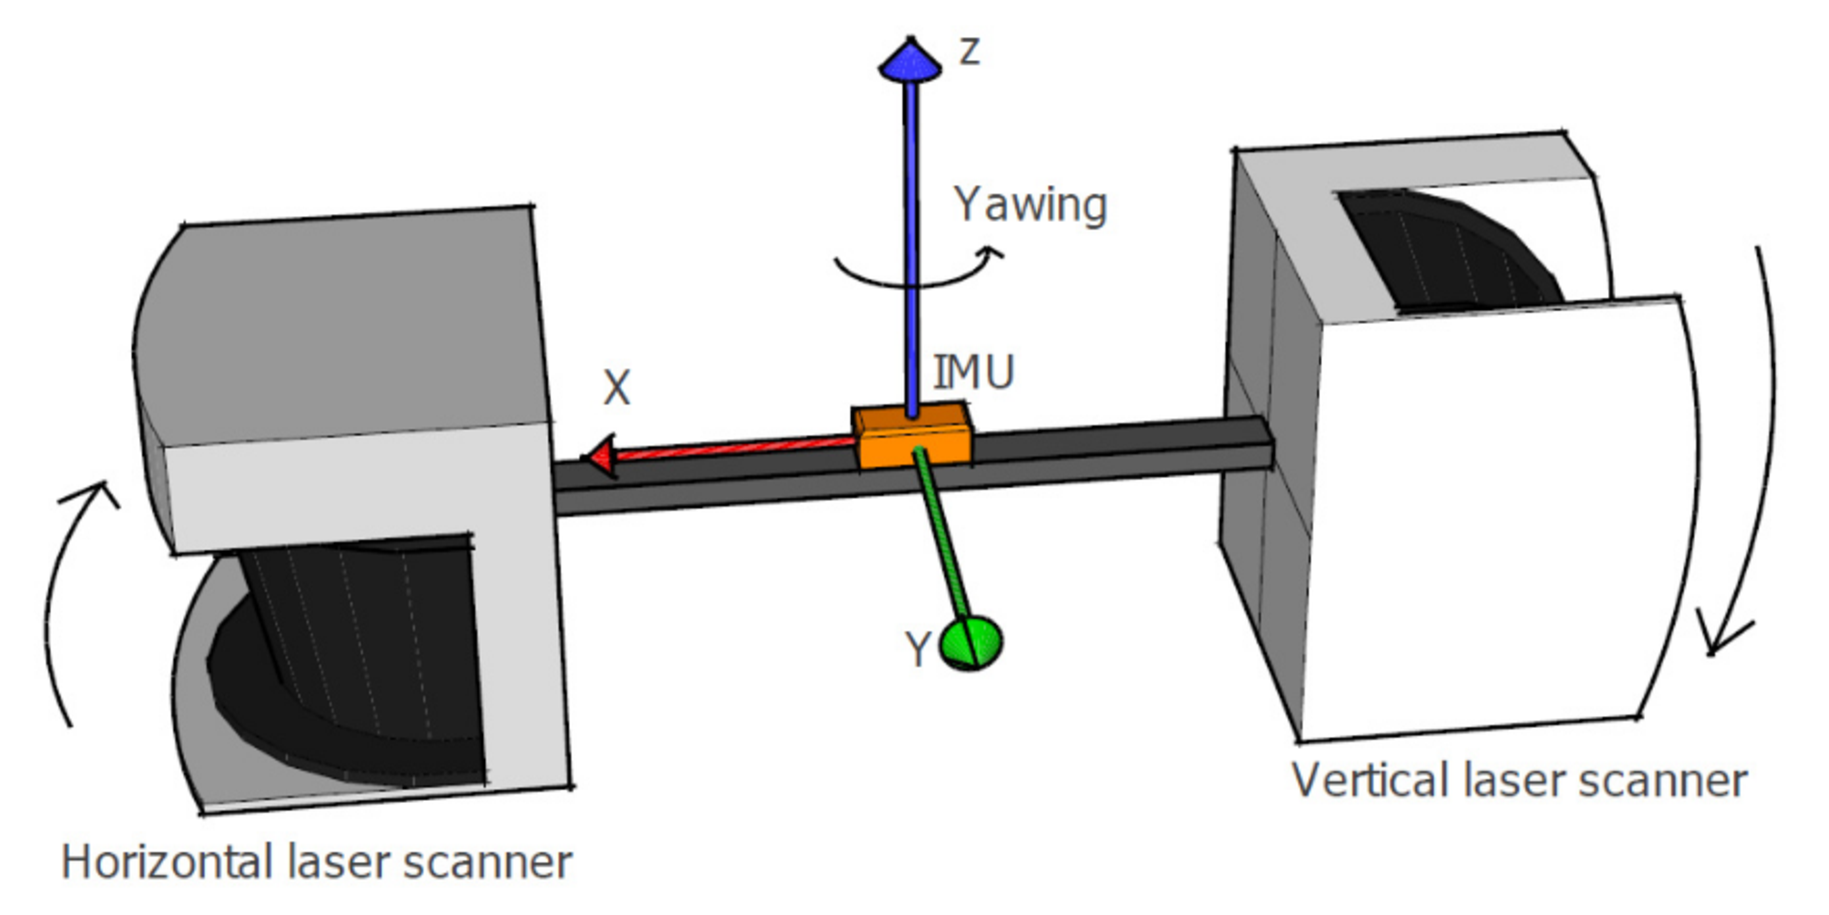
\includegraphics[width=0.5\textwidth]{graphics/laser_scanner_imu.eps}
  \caption{UAV mounted 3D scanner}
  \label{fig:laser_scanner_imu}
\end{figure}

This allows a point cloud describing the surroundings around the position of the
scanning system to be captured over several 2D scans as a series of point clouds
that are registered by first predicting their relative overlaps using IMU data
then using the Iterative Closest Point (ICP) algorithm \cite{Chen1992} to
perform fine registration.

This project demonstrates the ability to accurately register point clouds based
on the orientation of a sensor. As the core registration task is unchanged, this
workflow should also be applicable to point clouds captured from a 3D sensor
such as the Microsoft Kinect.

\subsection{Hypothesis}

This project aims to test the hypothesis that having recorded the position and
orientation of an RGB-D camera at the time of capture for a series of point
clouds, the complexity (as well as error in environments with little unique
features) of the registration process is greatly reduced.

This document will present the implementation of a point cloud capture and
registration application using a Microsoft Kinect and an IMU odometer for
position sensing, followed by an evaluation of each system in a series of test
cases aimed to stress the system.

\section{Experiment}

The hypothesis can be evaluated by implementing a point cloud capture system
that uses IMU odometry to replace the initial transformation guess that is
typically done using feature based methods such as key point finding using Scale
Invariant Feature Transform (SIFT) \cite{Lowe1999} and feature correspondences
using Fast Point Feature Histograms (FPFH) \cite{Rusu2009}.

The effectiveness of this approach can be simply evaluated by visual comparison
of the geometry shown by the captured point cloud with the actual geometry,
however a numerically quantifiable alternative can be taken as the difference
between the initial transformation guess provided by IMU odometry and the final
transformation.

A traditional feature based registration workflow will also be implemented and
the quality of registration can be compared over each workflow. The feature
based workflow will not have the use of IMU data as an initial estimate.

As the functionality of the IMU odometer is also a key component to this project
it will be evaluated separately from the point cloud manipulation portion of the
implementation.

Separate evaluation of the odometer also has the advantage of being a purely
numerical test of the performance of the odometer under a series of test cases
where the device will be actuated in a known way and the output of the odometer
compared to the known actuation.

\section{Implementation}

The implementation of the system used to evaluate the hypothesis can be broken
down to three key sections; the framework on which the capture and processing
application is built, the registration methods themselves and the IMU odometer
used to measure camera position and orientation.

\subsection{Conventions}

Unless otherwise noted the point type of a point cloud will be XYZ-RGBA, in
which the position is stored as three single precision floating point numbers
and the colour information and alpha channel are stored as 8 bit unsigned
integers (in PCL this is packed into an unsigned 32 bit integer).

When axes are being referred to with respect to an IMU then the axes orientation
of the IMU is used, this is shown by figure \ref{fig:mpu6000_axis_orientation}.
This axis orientation is the same for the MPU6000, MPU6050 and MPU9150. The X, Y
and Z axes may be referred to as the pitch, roll and yaw axes respectively.

The capture and processing application itself uses the left hand coordinate
system as shown in figure \ref{fig:application_axis_orientation}.

Conversion between coordinate systems used by the odometers and the application
are performed in the driver for the given device.

The units of length and time used throughout the implementation are metres and
seconds unless otherwise specified.

\begin{figure}[h!]
  \centering
  \begin{subfigure}[b]{0.4\textwidth}
    \centering
    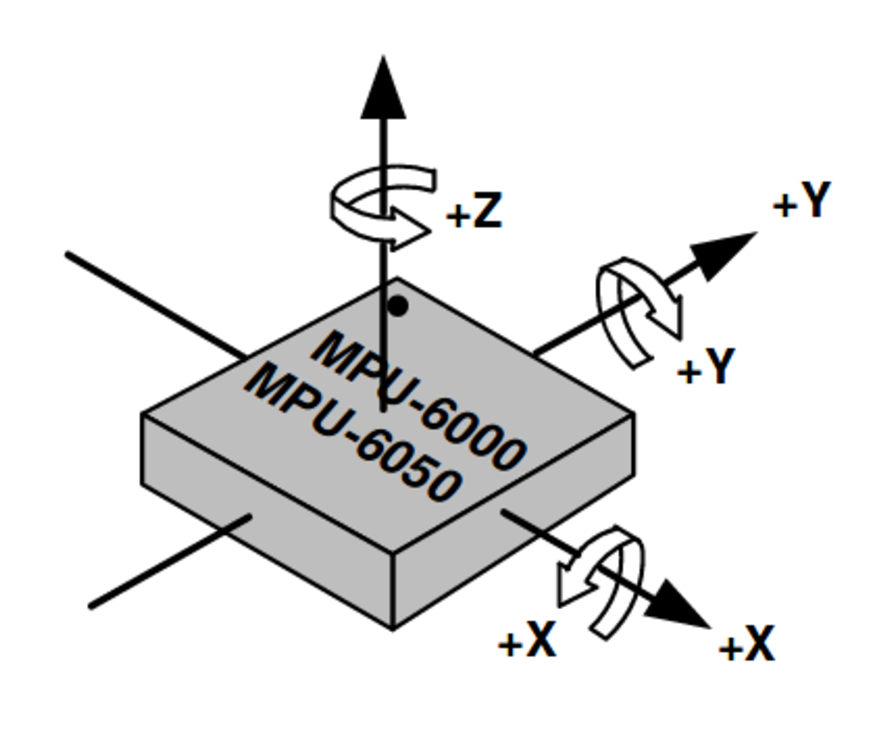
\includegraphics[width=0.6\textwidth]{graphics/mpu6000_axis_orientation.eps}
    \caption{IMU axis orientation \cite{mpu6000_datasheet}}
    \label{fig:mpu6000_axis_orientation}
  \end{subfigure}
  \begin{subfigure}[b]{0.4\textwidth}
    \centering
    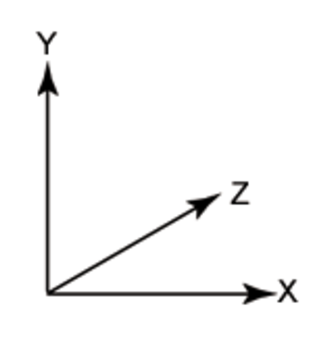
\includegraphics[width=0.4\textwidth]{graphics/application_coordinate_system.eps}
    \caption{Application axis orientation}
    \label{fig:application_axis_orientation}
  \end{subfigure}
  \caption{Axis systems used in this project}
\end{figure}

\subsection{Framework}
\label{sec:implementation_framework}

The initial task involved the implementation of a framework in which
implementations of various processing tasks could be produced. Ideally tasks
could be run either in real time or as a post processing step and should attempt
to make effective use of computational resourced on the host system.

The framework (as well as all processing methods, further described in section
\ref{sec:implementation_registration}) are implemented in C++ and built using
the CMake \cite{CMake} build system.

The implementation makes extensive use of the Point Cloud Library (PCL) which
provides stable framework for capturing, visualising and processing point
clouds.

\subsubsection{Libraries}

The \texttt{YukariCommon} library contains common functionality used throughout
the framework, this includes; the logging framework built upon spdlog, basic
data parsers and helper classes and functions.

\texttt{YukariMaths} contains a simple transformation representation with the
ability to be loaded and saved to a file. The majority of mathematical and
geometry functionality is provided by Eigen \cite{eigenweb} which is also
heavily used within PCL.

The \texttt{YukariTriggers} library provides a collection of event triggers that
may be used to trigger the capture of a new point cloud and IMU frame, if
applicable.

Triggers are used for either triggering a new frame capture or exiting the
capture application. The trigger interface provides a running/stopped state and
a callback for when a trigger event occurs.

\texttt{PeriodicTrigger} is a simple delay based trigger that calls the callback
function after a given amount of time has elapsed, this is the primary trigger
used when performing a capture operation.

\texttt{ProxyTrigger} provides a method of firing a trigger from any given
section of code, this is used internally for triggering processing operations
from saved point clouds.

\texttt{SignalTrigger} is typically used to exit the application on signal 2
(Ctrl-C).

\texttt{YukariIMU} provides the interface for capturing data from the IMU
odometer.

A class \texttt{IMUFrame} is used to represent a single capture form an IMU
odometer, this consist of a quaternion representing the orientation and a 3
element vector representing the displacement from the origin of the world (which
for all implemented IMU devices is the position it was in when was powered on or
the integrators were last reset).

This class also provides a conversion from the stored quaternion and vector to a
4x4 matrix including mirroring the orientation in the XZ plane. This is due to
the fact that when the camera "looks up" in the scene, the scene must be rotated
down to remain in the same orientation relative to the camera.

The implemented IMU grabbers are shown in figure \ref{fig:framework_imu}.

\texttt{ISerialGrabber} is an abstract class for IMU devices that communicate
over a serial port and handles parsing the serial port parameters and
opening/closing the port. \texttt{IMSPGrabber} adds an MSP client instance to
the serial port offered by \texttt{ISerialGrabber} for IMU devices that
communicate over MSP.

\texttt{MSPGrabberAttitude}, \texttt{TeensyIMUDevice} and
\texttt{STM32IMUDevice} and drivers for the "vanilla MSP", Teensy and STM32 IMU
devices respectively.

\texttt{FileIMUGrabber} is used to load saved IMU frames from disk and present
them as a stream of new IMU data where each read returns a frame loaded from the
next file in the sequence. This is used to facilitate post capture processing on
raw point clouds and IMU data.

\texttt{DummyIMUGrabber} is a random data generator used for testing.

\texttt{YukariMSP} is a helper library for parsing and generating MSP messages,
this is used in communication between the capture application and specific IMU
hardware.

The MSP protocol is a request-response based protocol, the format of which is
depicted in figure \ref{fig:msp_protocol}.

\begin{figure}[h!]
  \centering
  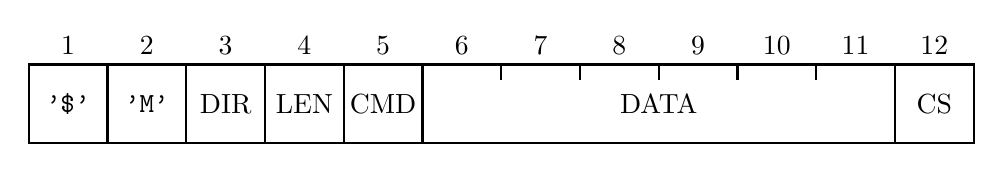
\begin{tikzpicture}
    \bitrect{12}{\bit}
    \rwbits{0}{1}{\texttt{'\$'}}
    \rwbits{1}{1}{\texttt{'M'}}
    \rwbits{2}{1}{DIR}
    \rwbits{3}{1}{LEN}
    \rwbits{4}{1}{CMD}
    \rwbits{5}{6}{DATA}
    \rwbits{11}{1}{CS}
  \end{tikzpicture}
  \caption{The MultiWii Serial Protocol (example for 6 byte payload)}
  \label{fig:msp_protocol}
\end{figure}

The first two bytes are a static header used to indicate the beginning of a data
frame, the third byte is used to indicate the direction of the message where
\texttt{<} denotes a message sent form the host to the external device and
\texttt{>} is a message from the device to the host.

The fourth byte is the length of the variable message data (i.e. the bytes
denoted by \texttt{DATA} in figure \ref{fig:msp_protocol}), the fifth byte
defines the command to be executed or the data that is contained in the payload.

The following $n$ bytes (where $n$ is provided by the \texttt{LEN} byte) is the
data payload and the final bye is a checksum of the data payload obtained by
XORing the \texttt{LEN}, \texttt{CMD} and payload bytes in order.

\texttt{YukariCloudCapture} provides the interface used to capture point clouds
for a implemented sources.

\texttt{PCLCloudGrabberWrapper} is a grabber that wraps a point cloud grabber
from the PCL framework (i.e. a subclass of \texttt{pcl::Grabber}).
\texttt{OPenNI2CloudGrabber} and \texttt{PCDFileCLoudGrabber} are
specialisations of this that define either a \texttt{pcl::io::OpenNI2Grabber},
for capturing point clouds from the Microsoft Kinect or a
\texttt{<pcl::PCDGrabber} for capturing point clouds from PCD data files.

The \texttt{DummyCloudGrabber} generates point clouds with randomly placed
points, this is intended for testing use.

Point cloud manipulation and processing tasks are implemented in the
\texttt{YukariProcessing} library.

Processing tasks are implemented in the \texttt{IFrameProcessingTask} interface
which provides queue functionality to hold jobs while processing is in progress.

\texttt{TaskDownsampleCloud} is a simple filter that uses a voxel grid to reduce
the density of a point cloud. This uses the \texttt{ApproximateVoxelGrid} filter
from PCL.

\texttt{TaskSaveRawCloud} and \texttt{TestSaveRawIMUFrame} are tasks that save
captured data to disk for debugging or post processing. The point cloud can
optionally be transformed by the IMU frame before saving.

\texttt{ITaskAlignment} is an abstract class for all processing tasks that
perform point cloud registration. The main functions of this class are parameter
parsing and configuration of PCL algorithms.

\texttt{ITaskIncrementalAlignment} and \texttt{ITaskWorldAlignment} are abstract
classes that implement the two registration methods as described in section
\ref{sec:implementation_registration}. Each registration method then subclasses
these abstract classes to implement the registration function.

In the case of triggers, IMU grabbers, cloud capture sources and processing
stages there are factories implemented that will create instances of each object
given a string defining the parameters to the specific implementation.

Factories accept strings in the format \textit{command(arg1=value1,
arg2=value2)}, these strings are parsed and presented to the factories as a map
of string parameters.

\subsubsection{Executables}

The \texttt{Capture} program is the main way scanning and processing is
performed within the framework. This is a command line program that accepts a
point cloud source, IMU data source, capture and exit trigger and any number of
processing tasks as parameters.

Each processing task added will run on its own worker thread and process frames
as they arrive as described in section \ref{sec:implementation_framework}.

\texttt{PCDViewer} is a copy of the point cloud viewer distributed in the PCL
source code \cite{PCLPCDViewer}. A copy is kept in the framework for
convenience given that not all binary distributions of PCL include this tool.

\texttt{CloudGrabberTest} is used for testing the point cloud grabber. When
executed this opens a point cloud grabber and shows every newly captured cloud
in a navigable graphical scene as they are captured. An IMU frame grabber can
also be provided in which case the cloud is transformed by the captured IMU
frame, this can be useful for testing combinations of point cloud grabber and
IMU grabbers.

\texttt{IMUGrabberTest} is used to test an IMU odometer. This shows a graphical
representation of the IMU odometer on screen and updates its position and
orientation according to the IMU frames captured by the device. This also allows
calibration of the accelerometer and magnetometer as well as integrator reset on
certain IMU devices.

\texttt{TriggerTest} is a command line program that shows when a given trigger
has been activated, this is mainly used as a debugging program and serves no
real purpose.

\subsection{Registration}
\label{sec:implementation_registration}

The registration of two point clouds involves determining areas of identical
geometry between them, in this instance it is recognising when two point clouds
describe the same scanned geometry (i.e. they overlap).

For the scope of this project we will only be concerned with registration of
pairs of point clouds and determining a ridged transformation between them.

Most registration methods denote the "existing" point cloud as the target and
the "new" point cloud as the input. It is the input cloud that is mapped onto
the target.

\subsubsection{Incremental vs. World}

There are two overarching methods of alignment that are implemented in the
framework; incremental registration as shown by figure
\ref{fig:incremental_alignment_workflow} and world registration as shown by
figure \ref{fig:world_alignment_workflow}.

Incremental registration operates by registering the last two captured point
clouds after each new frame and storing the transformation that maps the two on
top of each other.

This allows the clouds to be loaded, transformed and combined into a single
point cloud describing the full scanned geometry after the capture has been
completed.

\begin{figure}[h!]
  \centering
  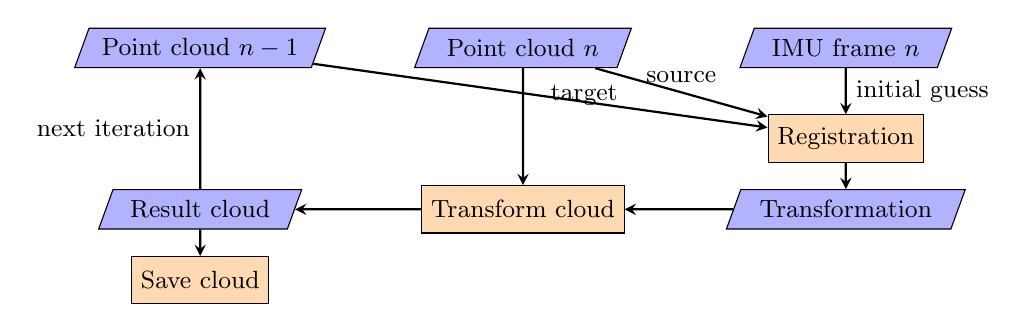
\begin{tikzpicture}[node distance=0.9cm]
    \node (point-cloud) [io] {Point cloud $n$};
    \node (imu-frame) [io, right of=point-cloud, xshift=3.2cm] {IMU frame $n$};
    \node (last-point-cloud) [io, left of=point-cloud, xshift=-3.2cm] {Point cloud $n-1$};
    \node (registration-method) [process, below of=imu-frame, yshift=-0.25cm] {Registration};
    \node (result-transform) [io, below of=registration-method] {Transformation};
    \node (transform) [process, left of=result-transform, xshift=-3.2cm] {Transform cloud};
    \node (result-cloud) [io, left of=transform, xshift=-3.2cm] {Result cloud};
    \node (save-cloud) [process, below of=result-cloud] {Save cloud};

    \draw [arrow] (last-point-cloud) -- node[anchor=west] {target} (registration-method);
    \draw [arrow] (point-cloud) -- node[anchor=south] {source} (registration-method);
    \draw [arrow] (imu-frame) -- node[anchor=west] {initial guess} (registration-method);
    \draw [arrow] (registration-method) -- (result-transform);
    \draw [arrow] (result-transform) -- (transform);
    \draw [arrow] (point-cloud) -- (transform);
    \draw [arrow] (transform) -- (result-cloud);
    \draw [arrow] (result-cloud) -- node[anchor=east] {next iteration} (last-point-cloud);
    \draw [arrow] (result-cloud) -- (save-cloud);
  \end{tikzpicture}
  \caption{Incremental registration workflow}
  \label{fig:incremental_alignment_workflow}
\end{figure}

The alternative is world registration, in which a point cloud describing the
world is kept in memory at all times during the capture process and each new
point cloud captured is aligned to this world cloud, transformed and
immediately appended to it.

\begin{figure}[h!]
  \centering
  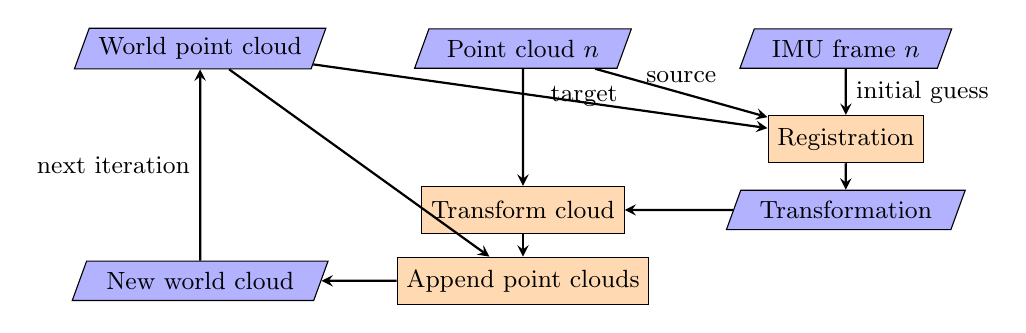
\begin{tikzpicture}[node distance=0.9cm]
    \node (point-cloud) [io] {Point cloud $n$};
    \node (imu-frame) [io, right of=point-cloud, xshift=3.2cm] {IMU frame $n$};
    \node (world-point-cloud) [io, left of=point-cloud, xshift=-3.2cm] {World point cloud};
    \node (registration-method) [process, below of=imu-frame, yshift=-0.25cm] {Registration};
    \node (result-transform) [io, below of=registration-method] {Transformation};
    \node (transform) [process, left of=result-transform, xshift=-3.2cm] {Transform cloud};
    \node (append-clouds) [process, below of=transform] {Append point clouds};
    \node (new-world-cloud) [io, left of=append-clouds,xshift=-3.2cm] {New world cloud};

    \draw [arrow] (world-point-cloud) -- node[anchor=west] {target} (registration-method);
    \draw [arrow] (point-cloud) -- node[anchor=south] {source} (registration-method);
    \draw [arrow] (imu-frame) -- node[anchor=west] {initial guess} (registration-method);
    \draw [arrow] (registration-method) -- (result-transform);
    \draw [arrow] (result-transform) -- (transform);
    \draw [arrow] (point-cloud) -- (transform);
    \draw [arrow] (transform) -- (append-clouds);
    \draw [arrow] (append-clouds) -- (new-world-cloud);
    \draw [arrow] (world-point-cloud) -- (append-clouds);
    \draw [arrow] (new-world-cloud) -- node[anchor=east] {next iteration} (world-point-cloud);
  \end{tikzpicture}
  \caption{World registration workflow}
  \label{fig:world_alignment_workflow}
\end{figure}

World registration has a distinct advantage to incremental registration in that
it does not matter what part of the already captured geometry a new frame
overlaps with as it will be registered against all known geometry. The only
requirement is that there is overlap with known geometry.

With incremental registration it is required that each new point cloud captured
overlaps with the last point cloud to be captured.

Incremental registration has the advantage of requiring the least memory and
computation to perform the registration, as the size of the target point cloud
is a constant size that is limited to the resolution of a single point cloud
capture and it is not required to have more than two full resolution point
clouds in memory at one time (i.e. the captured point cloud and the point cloud
captured in the previous frame).

As the registration method is not  can be used with any registration algorithm
the two workflows are implemented in two abstract classes. The registration of
a newly captured point cloud is performed by the
\texttt{ITaskAlignment::doAlignment()} virtual function which is implemented in
each registration class.

It is possible to combine the strengths of both of these approaches in a hybrid
registration method that operates on subsections of the world, this is further
discussed in section \ref{sec:further_work_hybrid_registration}.

\subsubsection{Input filtering}
\label{sec:input_filtering}

Before point clouds are registered there are three filtering stages applied to
them to improve the speed and quality of the registration.

The first is to remove any non numerical (NaN) values from the point cloud.

Non numerical values typically originate from sensor error during the capture
process. In the case of the Microsoft Kinect this would mean a depth "pixel"
giving an out of range reading, either due to too little detected infrared light
(for example the target is too far away or one part of the depth sensing optics
is obscured) or too much infrared light detected (for example in areas of high
ambient IR light).

Certain algorithms implemented in PCL seemed to cause problems when datasets
containing NaN values were used, performing this step removes the chance of such
issues occurring.

This also reduces the size of the data files generated by the capture process,
ideally there would be very few cases of NaN values in a captured point cloud
however the removal of them is still a small optimisation.

The second step is to remove any points which are determined to be outliers or
error. This is done using statistical analysis on a point and its neighbours.

The distances between a point and each point in its neighbourhood are
considered. In a situation with little error the distribution of these distances
is expected to be a Gaussian function. By specifying the shape of this Gaussian
points that do not fit within a tolerance of the expected distribution can be
assumed to be noise and removed from the point cloud.

This outlier removal filter can be toggled on and off as required.

The implementation of this filter is provided by
\texttt{pcl::StatisticalOutlierRemoval}.

In order to reduce the time taken for certain registration operations a
downsampling step is used which effectively reduces the density of the point
cloud.

This downsampling is performed using a voxel grid in which the world is split
into equal sized axis aligned cubes. For each cube (voxel) that contains points
its average is computed as the centroid of the points contained by it. The
downsampled point cloud is then constructed from the average points of all
non-empty voxels.

This downsampling is provided by the PCL implementation \texttt{pcl::VoxelGrid}.

\subsubsection{Iterative Closest Point (ICP)}

The Iterative Closest Point (ICP) \cite{Besl1992} is a registration algorithm
based on matching pairs of point between the input and target point clouds and
minimising the sum of the distance between all pairs.

The general workflow of the ICP algorithm is as follows \cite{Rusinkiewicz2001}:
\begin{enumerate}
  \item[1]
    Selecting a subset of the points in the input and target point clouds to be
    used for registration

  \item[2]
    Matching points between the two point clouds, in the most basic form this
    involves selecting the closest point from the target cloud for each point in
    the input cloud

  \item[3]
    Assigning a weight to pairs of matched points, this weight describes how
    well the points in each pair relate to each other

  \item[4]
    Reject matched pairs that are likely to be statistical outliers

  \item[5]
    Calculate an error metric describing the quality of the transformation
    between the point clouds

  \item[6]
    Iterate over steps two to five whilst making changes to the transformation
    of the input cloud relative to the target cloud in order to minimise the
    error metric

\end{enumerate}

In the case of this project the first selection step is performed by the voxel
filter described in section \ref{sec:input_filtering}.

The PCL implementation (\texttt{pcl::IterativeClosestPoint}) was used in this
project.

\subsubsection{Normal Distributions Transform (NDT)}

The Normal Distributions Transform (NDT) is a method of statistical registration
of point clouds presented by Biber and Stra{\ss}er \cite{Biber2003} for use with
2D range scans, later expended into 3D by Magnusson \cite{Magnusson2008}.

This approach starts by dividing the target world into cells of a constant size
and for each cell calculating the probability that a given point would be
measured in this cell.

This representation of the 3D point cloud provides a simple numerical
representation of the complex 3D space in the form of a probability
distribution.

The input point cloud is first transformed by an initial guess if one is
available, in this case this is provided by IMU odometery.

An iterative process then starts to minimise the total registration score, this
score is determined using the probability distributions of each cell in the
target world and the associated distribution for each sample of the input would
that is inside it.

After each iteration the transformation between the target and input world is
altered in order to find the optimal score, which in turn defines the most
likely registration between the two point clouds.

The stopping criteria are either a maximum number of iterations, the change in
score falling below a threshold (indicating convergence) or the difference in
parameters falling below a threshold (indicating convergence).

The PCL implementation (\texttt{pcl::NormalDistributionsTransform}) was used in
this project.

\subsubsection{Hybrid NDT/ICP}

Given that NDT registration does not need as accurate initial transformation
estimate as ICP it is possible to first register the two point clouds with NDT
to obtain a more accurate transformation estimate for ICP.

This method helps to guard against cases there the error in IMU reported data
would typically cause ICP registration to fail, which is most often due to
converging on a local minima.

In cases where the IMU informed estimate is of good quality then both
registration algorithms should exit after few iterations, therefore this hybrid
workflow should not add severe processing delay.

\subsubsection{Feature based initial transformation estimate}
\label{sec:feature_based_transform_estimate}

A traditional feature based registration workflow was implemented for comparison
with the IMU informed registration results. This workflow is described by
figures \ref{fig:feature_informed_registration_workflow_1} and
\ref{fig:feature_informed_registration_workflow_2}.

The process is split into two stages; a pre-processing stage that is performed
on a single point cloud to obtain a filtered copy of the point cloud and a set
of features describing it, and a registration stage that calculates a
transformation estimate using correspondences between the two point clouds and
performs a fine alignment using ICP.

The post processing stage is depicted by figure
\ref{fig:feature_informed_registration_workflow_1}. The first three steps are
filtering steps described in section \ref{sec:input_filtering}.

As point normals are required for feature estimation, a normal estimation step
is performed. This is essentially a plane fitting problem for a selection of
points in the neighbourhood of a target point.

This solves the direction of the plane normal but not its sign (i.e. which side
of the plane the normal faces). As there is no simple method of solving this it
is assumed the normal has which ever sign results in a direction closest towards
the viewpoint.

The radius of the neighbourhood for a given point plays an important part in
the normal estimation. The most common issue arising with a radius that is too
large for the scale or complexity of the point cloud, this can result in normals
that have contributions for adjacent surfaces and therefore do not properly
represent the edges of surfaces.

In this workflow the Fast Point Feature Histogram (FPFH)
\cite{Rusu_ICRA2011_PCL} representation was used to determine features of the
point clouds.

This method operates in the neighbourhood of each query point and categorises
the relationship between the query point and each point in the neighbourhood in
terms of the surface curvature as determined by the estimated surface normals.

These relationships are represented as a histograms for each query point of the
input point cloud.

The downsampled point cloud and feature cloud are stored for use in the second
stage of the workflow.

\begin{figure}[h!]
  \centering
  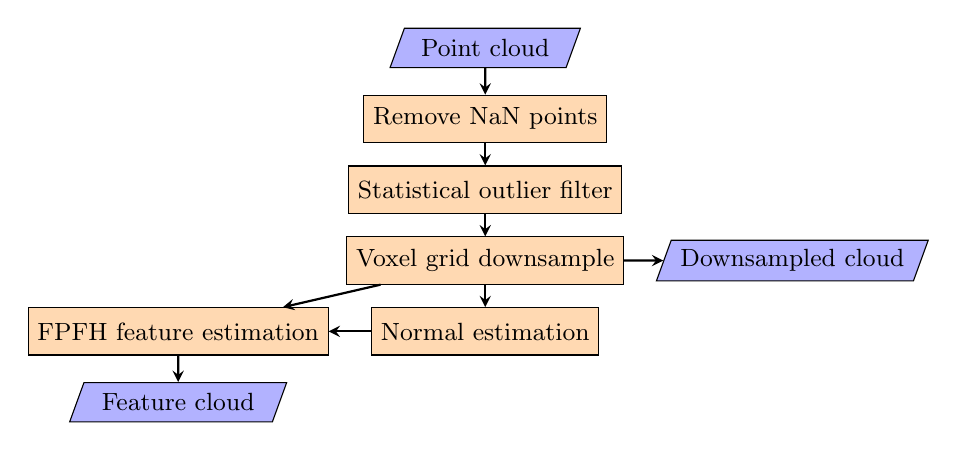
\begin{tikzpicture}[node distance=0.9cm]
    \node (cloud) [io] {Point cloud};
    \node (nan) [process, below of=cloud] {Remove NaN points};
    \node (filter) [process, below of=nan] {Statistical outlier filter};
    \node (downsample) [process, below of=filter] {Voxel grid downsample};
    \node (normal) [process, below of=downsample] {Normal estimation};
    \node (feature) [process, left of=normal, xshift=-3cm] {FPFH feature estimation};
    \node (downsample-cloud) [io, right of=downsample, xshift=3cm] {Downsampled cloud};
    \node (feature-cloud) [io, below of=feature] {Feature cloud};

    \draw [arrow] (cloud) -- (nan);
    \draw [arrow] (nan) -- (filter);
    \draw [arrow] (filter) -- (downsample);
    \draw [arrow] (downsample) -- (normal);
    \draw [arrow] (downsample) -- (feature);
    \draw [arrow] (normal) -- (feature);
    \draw [arrow] (downsample) -- (downsample-cloud);
    \draw [arrow] (feature) -- (feature-cloud);
  \end{tikzpicture}
  \caption{Feature informed registration: pre-processing step}
  \label{fig:feature_informed_registration_workflow_1}
\end{figure}

A set of correspondences are built by matching features from one cloud with the
closest matching feature from the other. This spatial search is carried out
using a kd-tree to reduce the complexity of the search operation.
\cite{Holz2015}

In the case of FPFH features, similarity matching is a fairly straightforward
difference between the feature histograms.

The next step is filtering out any erroneous correspondences which may
negatively effect the quality of the registration. This is done using RANSAC
\cite{Fischler1981} based approach.

A selection of correspondences are selected and a transformation that maps them
estimated. The source point cloud is then transformed by this estimation and any
correspondences with a Euclidean distance over a certain threshold are removed.

The downsampled point clouds are trimmed to only include points that are part of
a correspondence. This reduces the time taken for the fine registration step and
reduces the chances of a poor quality ICP optimisation.

There are several other documented methods of correspondence rejection, the
sample consensus method was chosen as it provides the best initial estimate
which is in important consideration when using ICP as the fine registration
algorithm. \cite{Holz2015}

Next the correspondences are used to estimate an initial transformation.
This is done using a singular value decomposition (SVD) based method described
by Horn \cite{Horn1987}.

The final step is to run a fine grained ICP registration using the trimmed point
clouds and the initial estimate derived from feature analysis.

In most cases only a small number of ICP iterations will be required for the
optimal transformation to be determined and the quality of the initial estimate
greatly reduces the change of the optimisation routine becoming stuck in a local
minima.

\begin{figure}[h!]
  \centering
  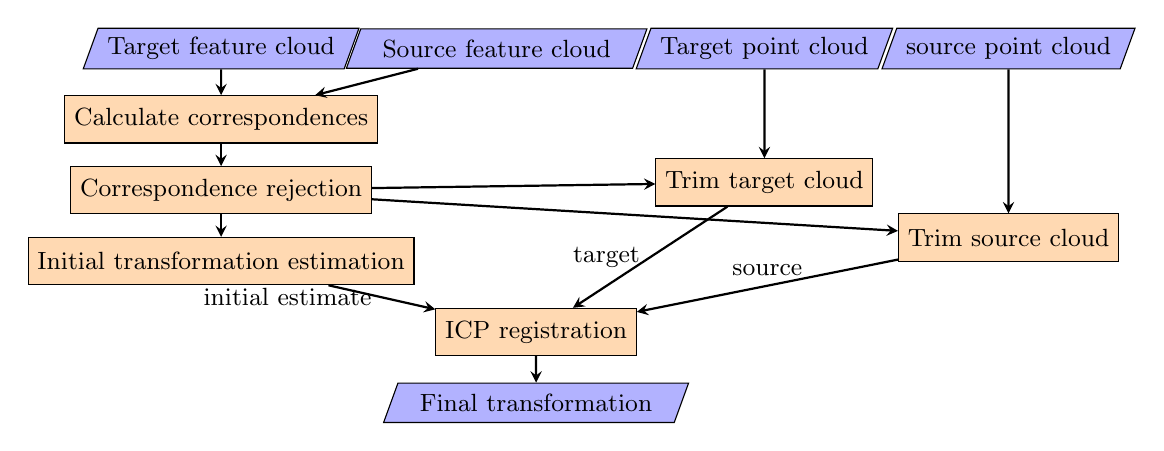
\begin{tikzpicture}[node distance=0.9cm]
    \node (target-feature-cloud) [io] {Target feature cloud};
    \node (source-feature-cloud) [io, right of=target-feature-cloud, xshift=2.6cm] {Source feature cloud};
    \node (correspondences) [process, below of=target-feature-cloud] {Calculate correspondences};
    \node (corr-reject) [process, below of=correspondences] {Correspondence rejection};
    \node (transform-est) [process, below of=corr-reject] {Initial transformation estimation};
    \node (icp) [process, below of=transform-est, xshift=4cm] {ICP registration};
    \node (transform-final) [io, below of=icp] {Final transformation};
    \node (target-cloud) [io, right of=source-feature-cloud, xshift=2.5cm] {Target point cloud};
    \node (source-cloud) [io, right of=target-cloud, xshift=2.2cm] {source point cloud};
    \node (trim-target) [process, below of=target-cloud, yshift=-0.8cm] {Trim target cloud};
    \node (trim-source) [process, below of=source-cloud, yshift=-1.5cm] {Trim source cloud};

    \draw [arrow] (target-feature-cloud) -- (correspondences);
    \draw [arrow] (source-feature-cloud) -- (correspondences);
    \draw [arrow] (correspondences) -- (corr-reject);
    \draw [arrow] (corr-reject) -- (transform-est);
    \draw [arrow] (transform-est) -- node[anchor=east] {initial estimate} (icp);
    \draw [arrow] (icp) -- (transform-final);
    \draw [arrow] (target-cloud) -- (trim-target);
    \draw [arrow] (source-cloud) -- (trim-source);
    \draw [arrow] (corr-reject) -- (trim-target);
    \draw [arrow] (corr-reject) -- (trim-source);
    \draw [arrow] (trim-target) -- node[anchor=east] {target} (icp);
    \draw [arrow] (trim-source) -- node[anchor=south] {source} (icp);
  \end{tikzpicture}
  \caption{Feature informed registration: registration step}
  \label{fig:feature_informed_registration_workflow_2}
\end{figure}

Given that this workflow uses analysis of the point cloud to inform the initial
estimation it should result in a good alignment assuming good parameters are
provided. This will form a good basis for comparison with the results of the IMU
informed registration workflows.

\subsection{Camera sensing}

The camera sensing component is an embedded device that is mounted to the camera
in order to accurately measure its position and orientation during each frame
capture.

Whilst the Microsoft Kinect does have an in built IMU this is only suited to
medium accuracy orientation measurements, for instance determining the angle of
the camera when operating the tilt motor.

\subsubsection{"Vanilla MSP"}

The first sensor implemented was an implementation of the MultiWii Serial
Protocol (MSP) typically used to communicate with flight control boards used
for small unmanned aerial systems, this was done as a quick proof of concept to
test orientation informed alignments before larger amounts of time were devoted
to implementation of an application specific IMU odometer.

Whist the API offered by MSP implementations differs greatly depending on the
firmware used on a given flight control board, almost all implementations allow
querying the yaw/pitch/roll angles of the board which was then converted to a
quaternion by the driver implemented in the capture framework.

Depending on the hardware present on the flight control board the yaw angle may
be an absolute heading (when a compass is present) or the angular displacement
since the device was powered on (in the case of a gyroscope and accelerometer
only).

This device has two significant flaws; it only senses orientation and the range
of orientation is limited, most notably an angle higher that roughly 60-70
degrees in pitch or roll axis would lead to erroneous results.

\subsubsection{Teensy 3.2 \& MPU9150}

This odometer is built using a Teensy 3.2 \cite{teensy32} development board
containing a Freescale ARM Cortex-M4 microcontroller (MK20DX256VLH7) and an
InvenSense MPU9150 IMU on a breakout board connected via the i2c interface.

The microcontroller is clocked at 72MHz and does not feature a hardware floating
point unit.

The MPU9150 is a 9 degrees of freedom IMU containing a 3 axis MEMS gyroscope, a
3 axis MEMS accelerometer and a 3 axis magnetometer.

The IMU features a coprocessor used to run the Digital Motion Processor software
to perform data fusion on chip, whilst this is available in a 9 DoF version to
include the magnetometer data this was not supported in the driver used to
communicate with the sensor. As a result data fusion was limited to 6 DoF, the
only noticeable impact this has is that the measured orientation is not
absolute whereas 9 DoF fusion would align the orientation with compass north.

The firmware for the microcontroller was written using the Arduino framework and
built using the PlatformIO tool chain.

Figure \ref{fig:teensy_mpu9150_imu_workflow} shows the data acquisition workflow
for the odometer, this is executed as each new frame of data from the DMP
arrives a at the microcontroller.

\begin{figure}[h!]
  \centering
  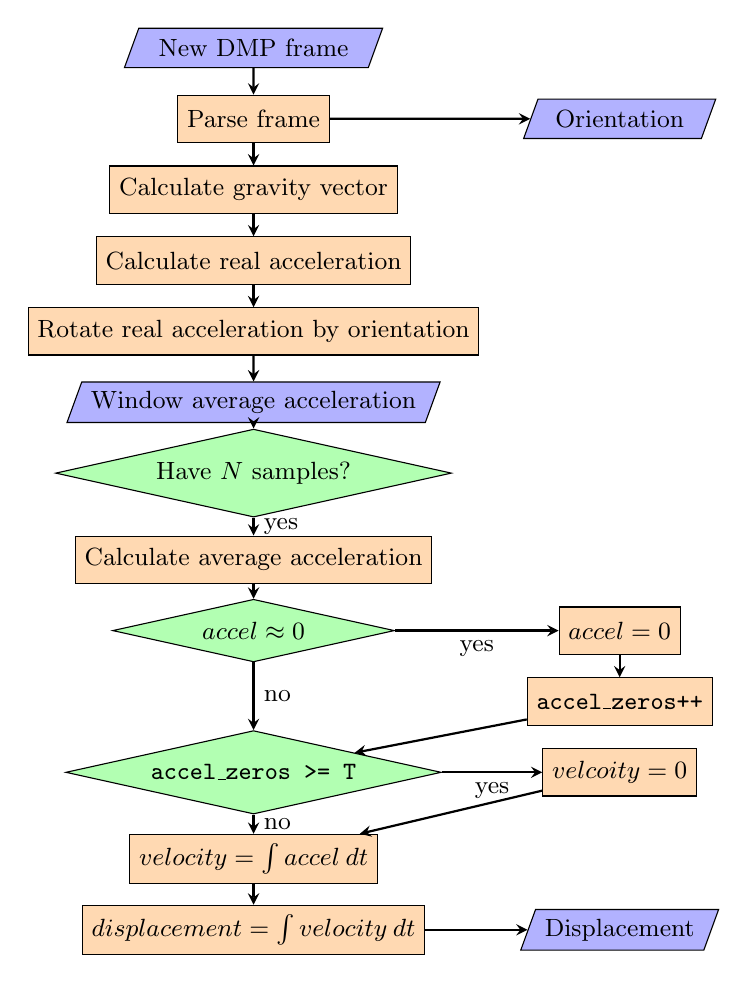
\begin{tikzpicture}[node distance=0.9cm]
    \node (dmp-frame) [io] {New DMP frame};
    \node (parse-dmp-frame) [process, below of=dmp-frame] {Parse frame};
    \node (orientation) [io, right of=parse-dmp-frame, xshift=3.75cm] {Orientation};
    \node (gravity-vector) [process, below of=parse-dmp-frame] {Calculate gravity vector};
    \node (real-accel) [process, below of=gravity-vector] {Calculate real acceleration};
    \node (rotate-accel) [process, below of=real-accel] {Rotate real acceleration by orientation};
    \node (accel-average) [io, below of=rotate-accel] {Window average acceleration};
    \node (accel-average-have-samples) [decision, below of=accel-average] {Have $N$ samples?};
    \node (accel-calc-average) [process, below of=accel-average-have-samples, yshift=-0.2cm] {Calculate average acceleration};
    \node (accel-close-to-zero) [decision, below of=accel-calc-average] {$accel \approx 0$};
    \node (set-accel-zero) [process, right of=accel-close-to-zero, xshift=3.75cm] {$accel = 0$};
    \node (increment-accel-zero-count) [process, below of=set-accel-zero] {\texttt{accel\_zeros++}};
    \node (spacer1) [below of=accel-close-to-zero] {};
    \node (accel-zero-count-check) [decision, below of=spacer1] {\texttt{accel\_zeros >= T}};
    \node (reset-velocity) [process, right of=accel-zero-count-check, xshift=3.75cm] {$velcoity = 0$};
    \node (integrate-accel) [process, below of=accel-zero-count-check, yshift=-0.2cm] {$velocity = \int accel \: dt$};
    \node (integrate-velocity) [process, below of=integrate-accel] {$displacement = \int velocity \: dt$};
    \node (displacement) [io, right of=integrate-velocity, xshift=3.75cm] {Displacement};

    \draw [arrow] (dmp-frame) -- (parse-dmp-frame);
    \draw [arrow] (parse-dmp-frame) -- (orientation);
    \draw [arrow] (parse-dmp-frame) -- (gravity-vector);
    \draw [arrow] (gravity-vector) -- (real-accel);
    \draw [arrow] (real-accel) -- (rotate-accel);
    \draw [arrow] (rotate-accel) -- (accel-average);
    \draw [arrow] (accel-average) -- (accel-average-have-samples);
    \draw [arrow] (accel-average-have-samples) -- node[anchor=west] {yes} (accel-calc-average);
    \draw [arrow] (accel-calc-average) -- (accel-close-to-zero);
    \draw [arrow] (accel-close-to-zero) -- node[anchor=north] {yes} (set-accel-zero);
    \draw [arrow] (accel-close-to-zero) -- node[anchor=west] {no} (accel-zero-count-check);
    \draw [arrow] (accel-zero-count-check) -- node[anchor=west] {no} (integrate-accel);
    \draw [arrow] (accel-zero-count-check) -- node[anchor=north] {yes} (reset-velocity);
    \draw [arrow] (reset-velocity) -- (integrate-accel);
    \draw [arrow] (set-accel-zero) -- (increment-accel-zero-count);
    \draw [arrow] (increment-accel-zero-count) -- (accel-zero-count-check);
    \draw [arrow] (integrate-accel) -- (integrate-velocity);
    \draw [arrow] (integrate-velocity) -- (displacement);
  \end{tikzpicture}
  \caption{Teensy 3.2 \& MPU9120 IMU workflow}
  \label{fig:teensy_mpu9150_imu_workflow}
\end{figure}

A quaternion representing the sensor orientation is extracted directly from the
DMP data frame.

The local device acceleration is extracted from the frame as a signed 16 bit
integer, this must then be scaled according to the accelerometer scale setting
(full scale acceleration on the MPU9150 can be either 2g, 4g, 8g or 16g).

A vector denoting the direction of gravity is then calculated from the
orientation quaternion.

This gravity vector is subtracted from the acceleration measured by the IMU to
obtain acceleration due to linear motion of the device. This is then rotated by
the orientation quaternion to give the linear acceleration in the world frame.

The world frame acceleration is then averaged over a number of samples to form a
rudimentary low pass filter (LPF).

When sufficient samples have been collected a check is performed in each axis of
the acceleration vector to see if the acceleration for a given axis is below a
threshold, if so the axis in question is set to zero.

A counter is kept to record how many consecutive zero readings have happened on
each axis of the world frame acceleration, if the count for a given axis reaches
a given threshold then it is assumed that the motion in that axis has ended and
the velocity for that axis is set to zero.

It is important that this threshold count is set correctly for the expected
motion of the odometer. For instance setting a low threshold when the odometer
will be exposed to long periods of movement at a constant speed would cause
misreported end of motion events. With sufficiently long movements this end of
movement test may not be appropriate at all as the threshold would become so
high it provides no benefit.

Given that the use of the point cloud capture system is expected to operate in a
high dynamics environment, i.e. exposed to frequent changes in acceleration,
this method of an end of movement check is suitable.

The world frame acceleration is then integrated another step to update the
velocity of the IMU. The velocity is then integrated to update the displacement.

This odometry workflow was based on the application note by NXP Semiconductor
\cite{NXP_AppNote_AN3397} which describes the process for two dimensional
odometry with the IMU constrained in a fixed plane perpendicular to the gravity
vector.

\subsubsection{STM32 \& MPU6000}

This IMU device was implemented in an attempt to obtain more reliable
displacement measurements from double integrated acceleration than what was
possible with the Teensy based IMU.

This device consists of an STM32F4 microcontroller and an InvenSense MPU6000 IMU
connected over Serial Peripheral Interface (SPI). The specific hardware used was
an Airbot Omnibus F4 flight control board, the small form factor of the board
and the fact it is a pre-made device makes this an idea choice for this
application.

The STM32F4 is an ARM Cortex M4 processor with a hardware floating point unit
running at 168 MHz, this combined with the higher data rate of the SPI bus
allows sampling the MPU6000 at the full 8 kHz allowed. This faster loop time
gives a finer integration time step and contributes to removing error in the
measured displacement.

The firmware for this device was written in C using the opencm3
\cite{libopencm3} hardware abstraction library for ARM Cortex microcontrollers.

Figure \ref{fig:stm32_mpu6000_imu_workflow} shows the data acquisition workflow
for the odometer, the loop is triggered on a periodic basis at 8 kHz to match
the sampling frequency of the IMU.

\begin{figure}[h!]
  \centering
  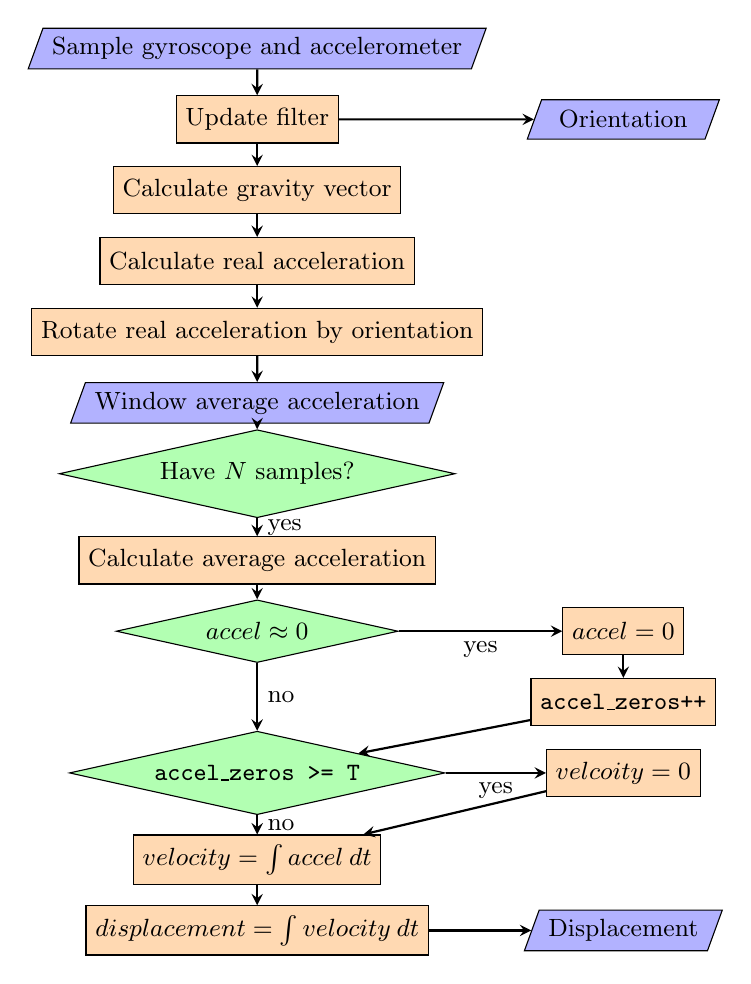
\begin{tikzpicture}[node distance=0.9cm]
    \node (sample) [io] {Sample gyroscope and accelerometer};
    \node (filter) [process, below of=sample] {Update filter};
    \node (orientation) [io, right of=filter, xshift=3.75cm] {Orientation};
    \node (gravity-vector) [process, below of=filter] {Calculate gravity vector};
    \node (real-accel) [process, below of=gravity-vector] {Calculate real acceleration};
    \node (rotate-accel) [process, below of=real-accel] {Rotate real acceleration by orientation};
    \node (accel-average) [io, below of=rotate-accel] {Window average acceleration};
    \node (accel-average-have-samples) [decision, below of=accel-average] {Have $N$ samples?};
    \node (accel-calc-average) [process, below of=accel-average-have-samples, yshift=-0.2cm] {Calculate average acceleration};
    \node (accel-close-to-zero) [decision, below of=accel-calc-average] {$accel \approx 0$};
    \node (set-accel-zero) [process, right of=accel-close-to-zero, xshift=3.75cm] {$accel = 0$};
    \node (increment-accel-zero-count) [process, below of=set-accel-zero] {\texttt{accel\_zeros++}};
    \node (spacer1) [below of=accel-close-to-zero] {};
    \node (accel-zero-count-check) [decision, below of=spacer1] {\texttt{accel\_zeros >= T}};
    \node (reset-velocity) [process, right of=accel-zero-count-check, xshift=3.75cm] {$velcoity = 0$};
    \node (integrate-accel) [process, below of=accel-zero-count-check, yshift=-0.2cm] {$velocity = \int accel \: dt$};
    \node (integrate-velocity) [process, below of=integrate-accel] {$displacement = \int velocity \: dt$};
    \node (displacement) [io, right of=integrate-velocity, xshift=3.75cm] {Displacement};

    \draw [arrow] (sample) -- (filter);
    \draw [arrow] (filter) -- (orientation);
    \draw [arrow] (filter) -- (gravity-vector);
    \draw [arrow] (gravity-vector) -- (real-accel);
    \draw [arrow] (real-accel) -- (rotate-accel);
    \draw [arrow] (rotate-accel) -- (accel-average);
    \draw [arrow] (accel-average) -- (accel-average-have-samples);
    \draw [arrow] (accel-average-have-samples) -- node[anchor=west] {yes} (accel-calc-average);
    \draw [arrow] (accel-calc-average) -- (accel-close-to-zero);
    \draw [arrow] (accel-close-to-zero) -- node[anchor=north] {yes} (set-accel-zero);
    \draw [arrow] (accel-close-to-zero) -- node[anchor=west] {no} (accel-zero-count-check);
    \draw [arrow] (accel-zero-count-check) -- node[anchor=west] {no} (integrate-accel);
    \draw [arrow] (accel-zero-count-check) -- node[anchor=north] {yes} (reset-velocity);
    \draw [arrow] (reset-velocity) -- (integrate-accel);
    \draw [arrow] (set-accel-zero) -- (increment-accel-zero-count);
    \draw [arrow] (increment-accel-zero-count) -- (accel-zero-count-check);
    \draw [arrow] (integrate-accel) -- (integrate-velocity);
    \draw [arrow] (integrate-velocity) -- (displacement);
  \end{tikzpicture}
  \caption{STM32 \& MPU6000 IMU workflow}
  \label{fig:stm32_mpu6000_imu_workflow}
\end{figure}

The workflow is largely similar to that used for the Teensy based odometer, the
only key difference is the method used to obtain the orientation.

To obtain the orientation from the raw IMU data the 6 DoF variant of the filter
described by Madgwick \cite{Madgwick2011}. This bases an initial estimate of the
orientation on the integrated angular velocity as measured by the gyroscope then
refines this estimate using a corrective step based on accelerometer data.

The filter is tuned using a single parameter $\beta$ which is used to correct
for error in the raw gyroscope measurements, essentially this parameter controls
how much of an influence the accelerometer correction step has on the resulting
orientation.

\section{Evaluation}

This section aims to critically evaluate the performance of the implemented
system in several test scenarios based on situations where its performance
should theoretically be an improvement on existing systems.

For instance, an initial registration transformation from IMU odometery has
potential to provide a better starting point that an initial transformation from
feature based techniques in areas of few distinct features.

\subsection{Point cloud registration}

This section evaluates the performance of the implemented registration methods
that follow the IMU informed workflow.

The quality of registration is determined by visual inspection of the resulting
point cloud alone. Originally this was going to be done by comparison to
registration using a feature informed initial estimate, however this could not
be made top operate reliably enough for this purpose. This is discussed further
in section \ref{sec:feature_informed_registration}.

With the exception of the first room scan only the highest quality registration
is mentioned for each test scenario.

Differences in surface colour are to be expected as the change in orientation of
the camera may result in a sufficient change in conditions to alter the
automatic RGB camera parameters (most notably exposure). As such these changes
in colour are not a sign of a bad registration.

\subsubsection{Feature informed registration}
\label{sec:feature_informed_registration}

The feature based initial estimation workflow performed very well when the
correct parameters for a given environment were found, unfortunately
determining these parameters proved difficult in most cases and a lot of the
attempted registrations resulted in wildly incorrect transformations.

Figure \ref{fig:room_1_transformed} shows a collection of five captured point
clouds with only the IMU obtain transformation applied. Due to the error in the
IMU measurement there are noticeable misalignments, these can be seen most on
sharp edges such as the chair, door and cabinet edges.

\begin{figure}[h!]
  \centering
  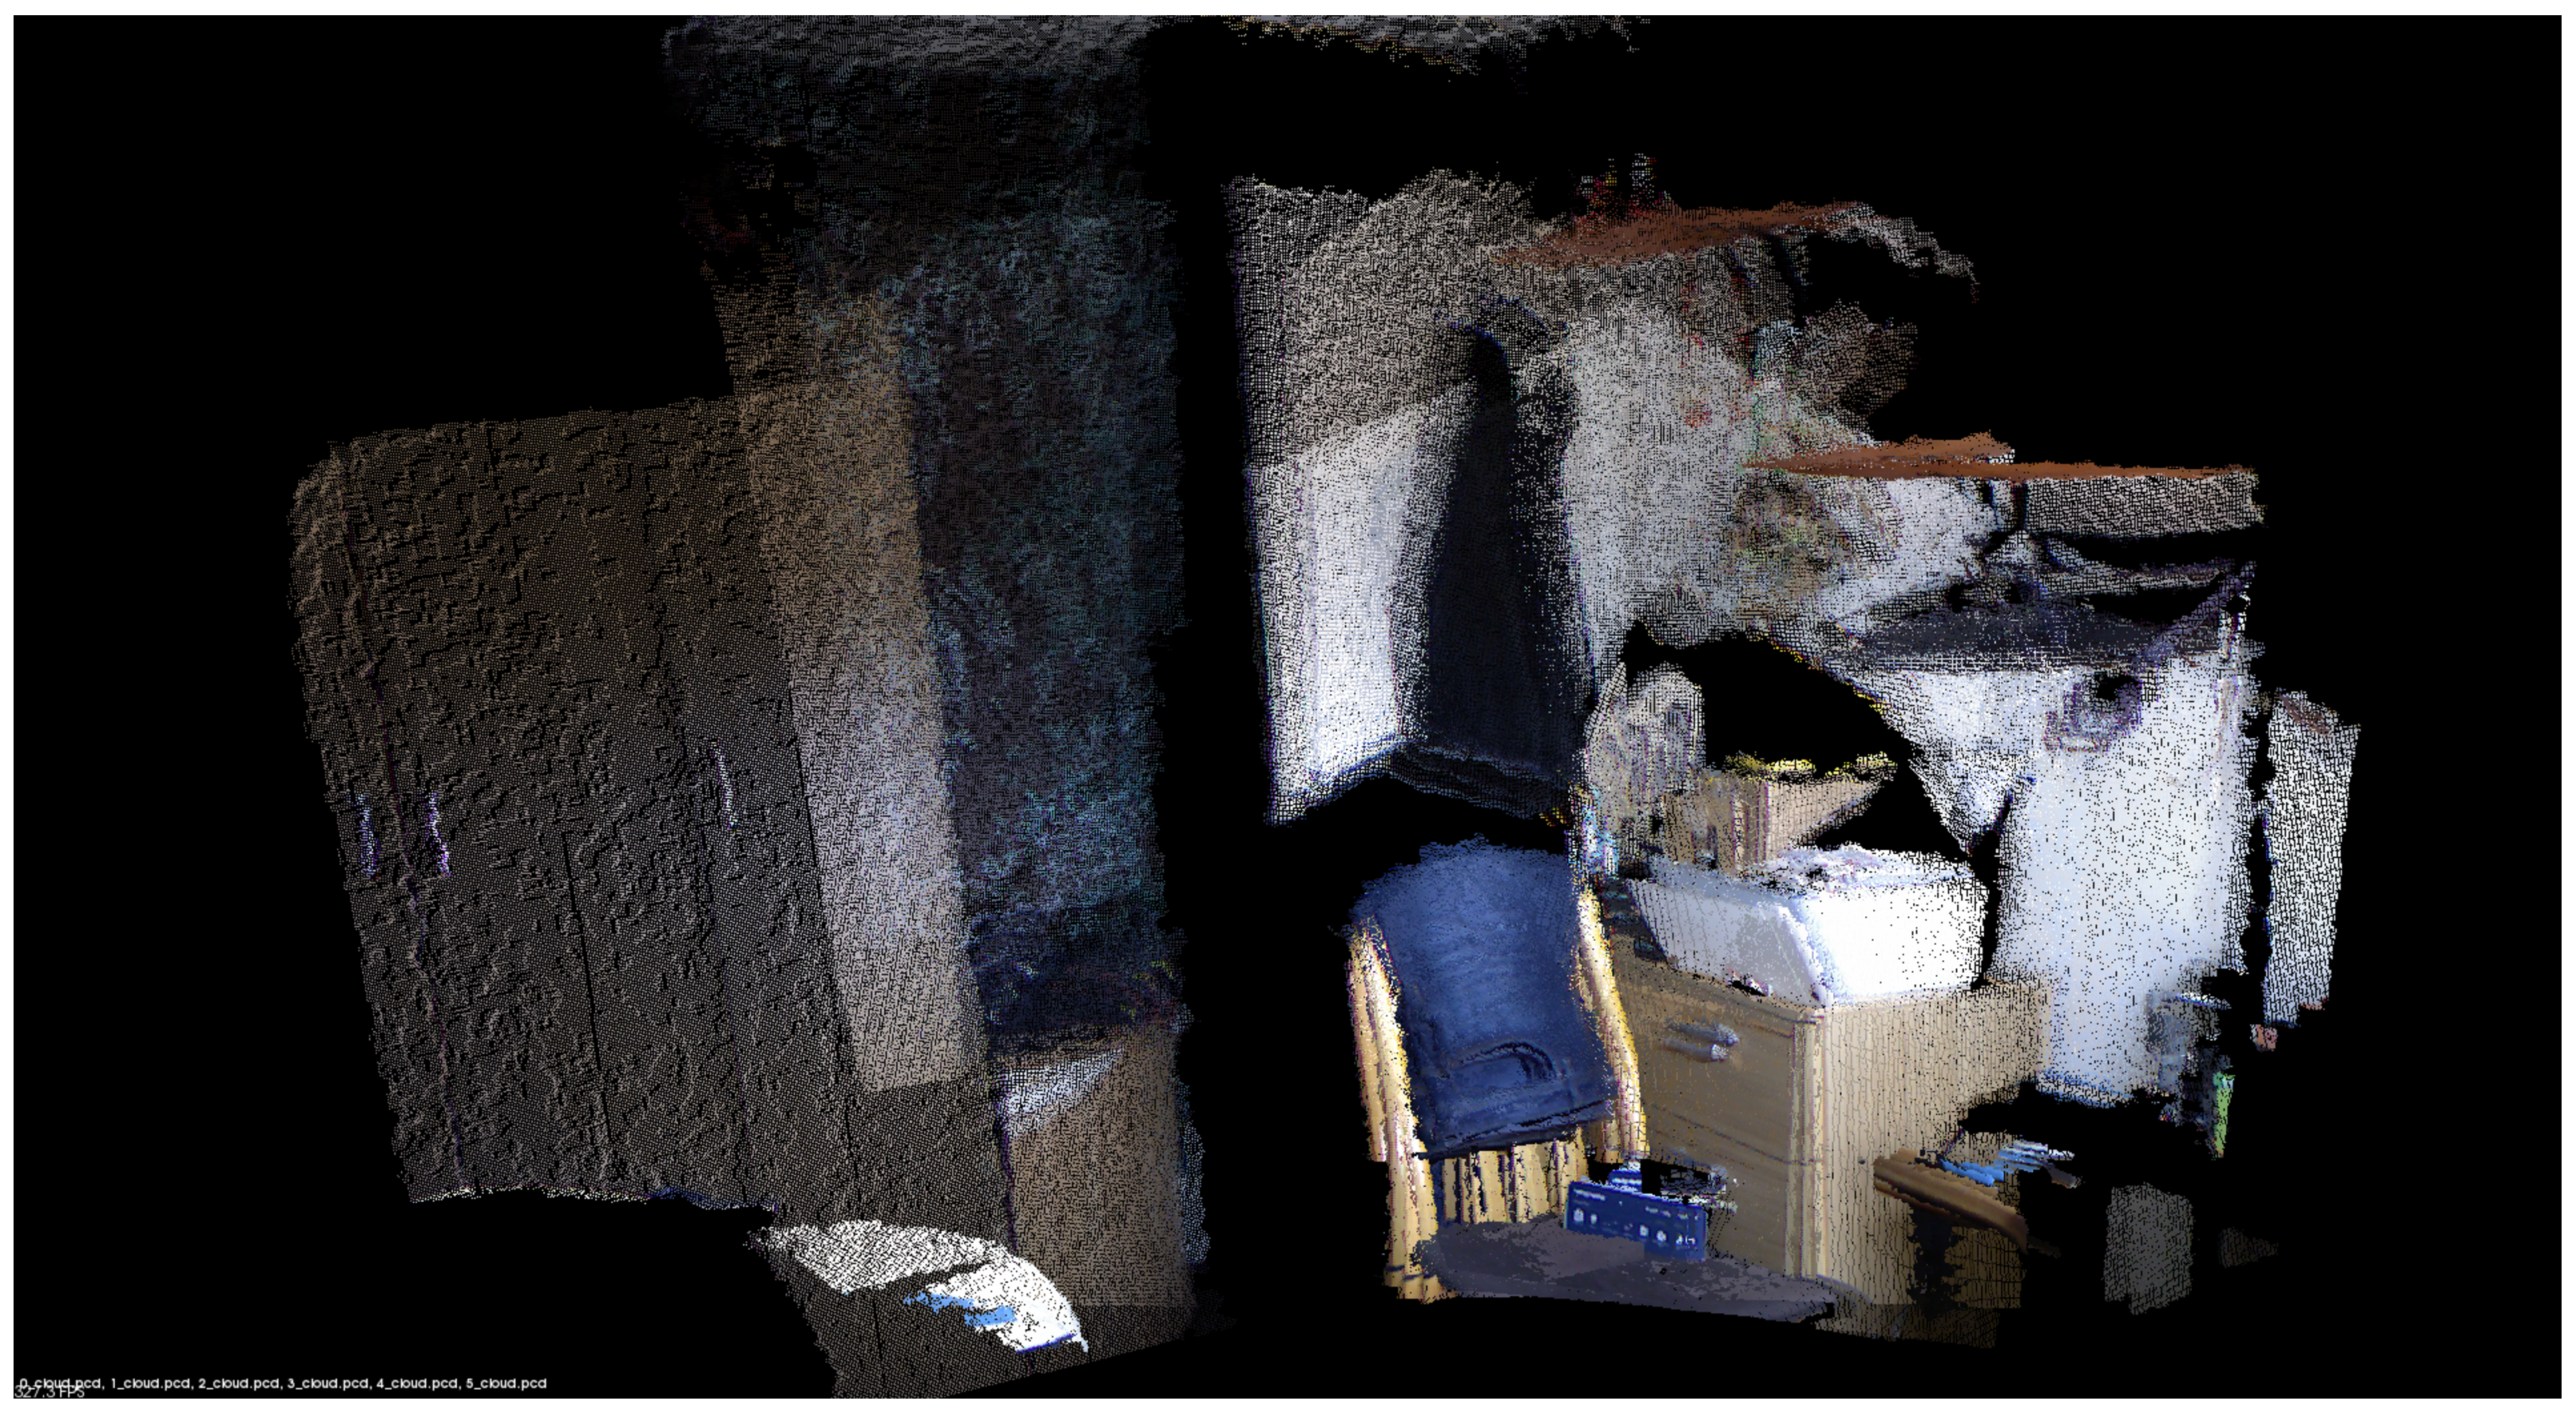
\includegraphics[width=0.7\textwidth]{graphics/room_1_transformed.eps}
  \caption{Room scan 1 transformed cloud}
  \label{fig:room_1_transformed}
\end{figure}

Figure \ref{fig:room_1_feature} shows two of the point clouds form this room
scan aligned using the workflow described in section
\ref{sec:feature_based_transform_estimate}.

This provided a very good initial transformation estimate which needed very
little refinement though ICP. There are no obvious visual alignment artefacts in
the registered point cloud.

\begin{figure}[h!]
  \centering
  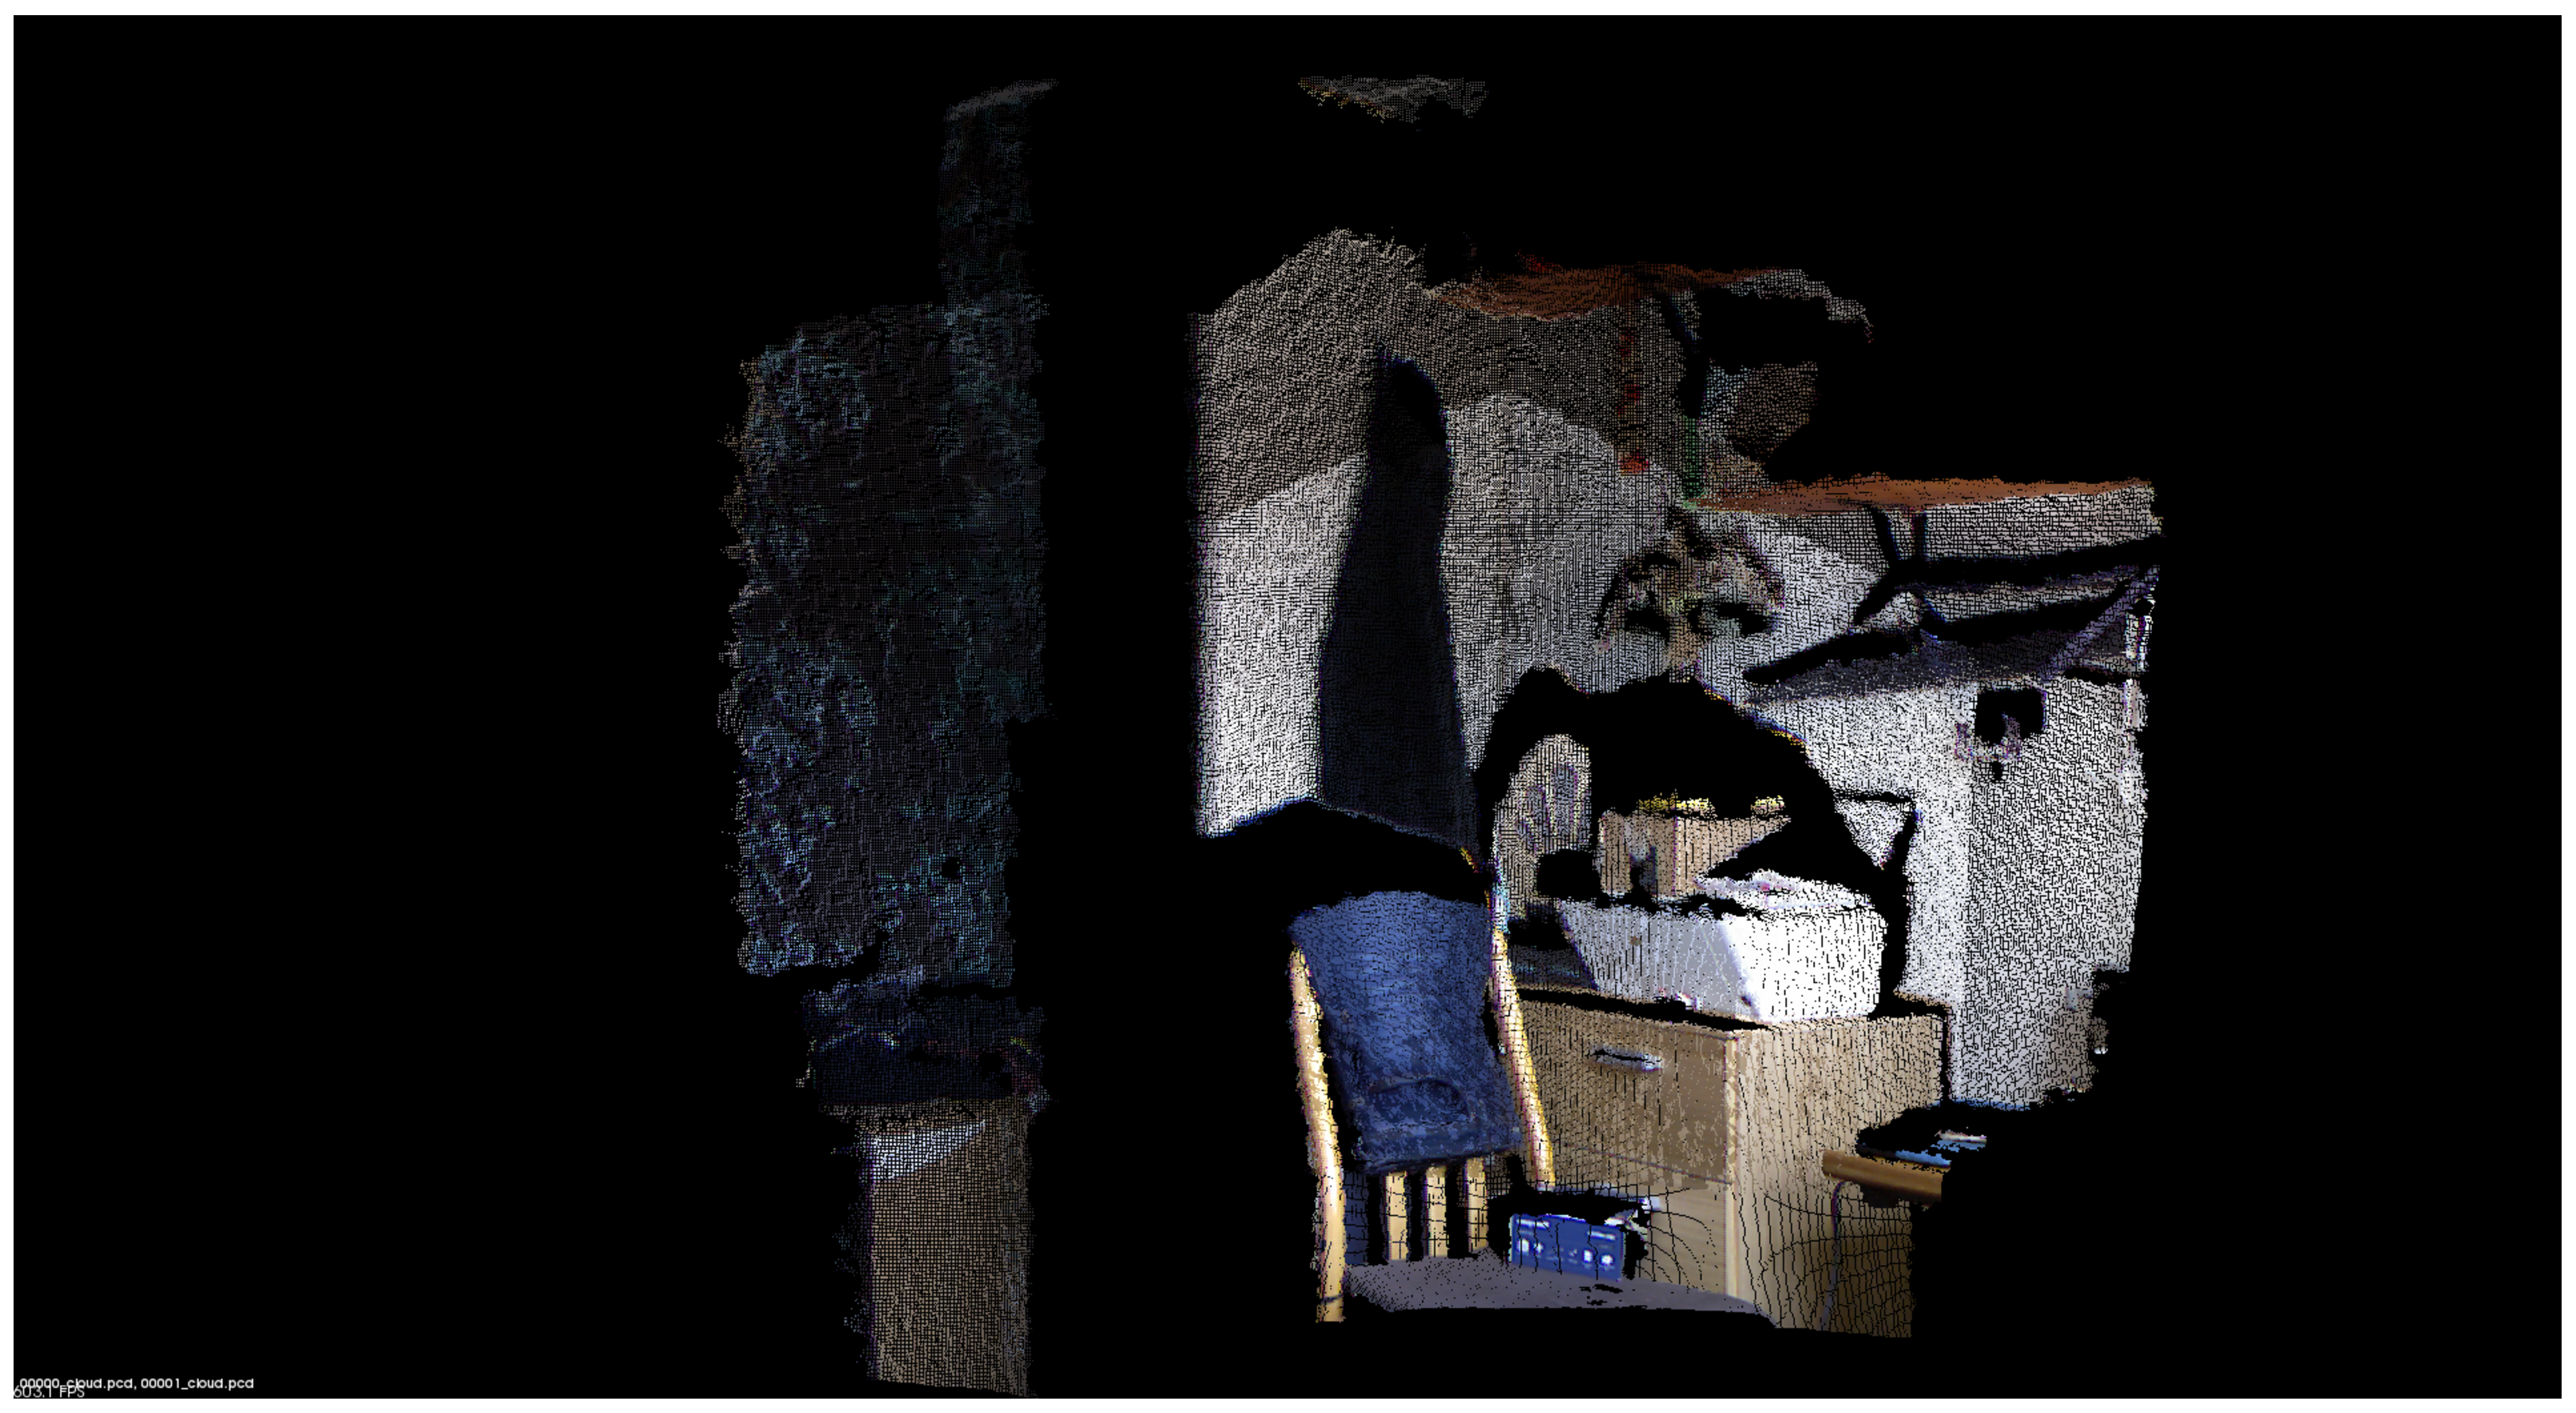
\includegraphics[width=0.7\textwidth]{graphics/room_1_feature.eps}
  \caption{Room scan 1 feature registered cloud}
  \label{fig:room_1_feature}
\end{figure}

This was the best feature based alignment that was obtained with the implemented
workflow. Theoretically there is no reason why this would not work well for
other collections of point clouds, however finding correct parameters to make
this possible proved difficult.

The effects of bad parameters often result in a registration that is very far
from the correct solution, usually due to a combination of incorrect
correspondences not being rejected and valid correspondences not being found.

A common cause of this is incorrect normal estimations, given that the surface
curvature and therefore the point normals are what the key point finding is
based upon.

\subsubsection{Medium range room scan}

Two scans were used at medium sized room scale. The first in a narrow field of
view and the second over a wider field of view with less overlap between
adjacent point cloud captures.

Figure \ref{fig:room_1_ndt} shows the point clouds from the previous section
registered using the NDT based world alignment workflow.

\begin{figure}[h!]
  \centering
  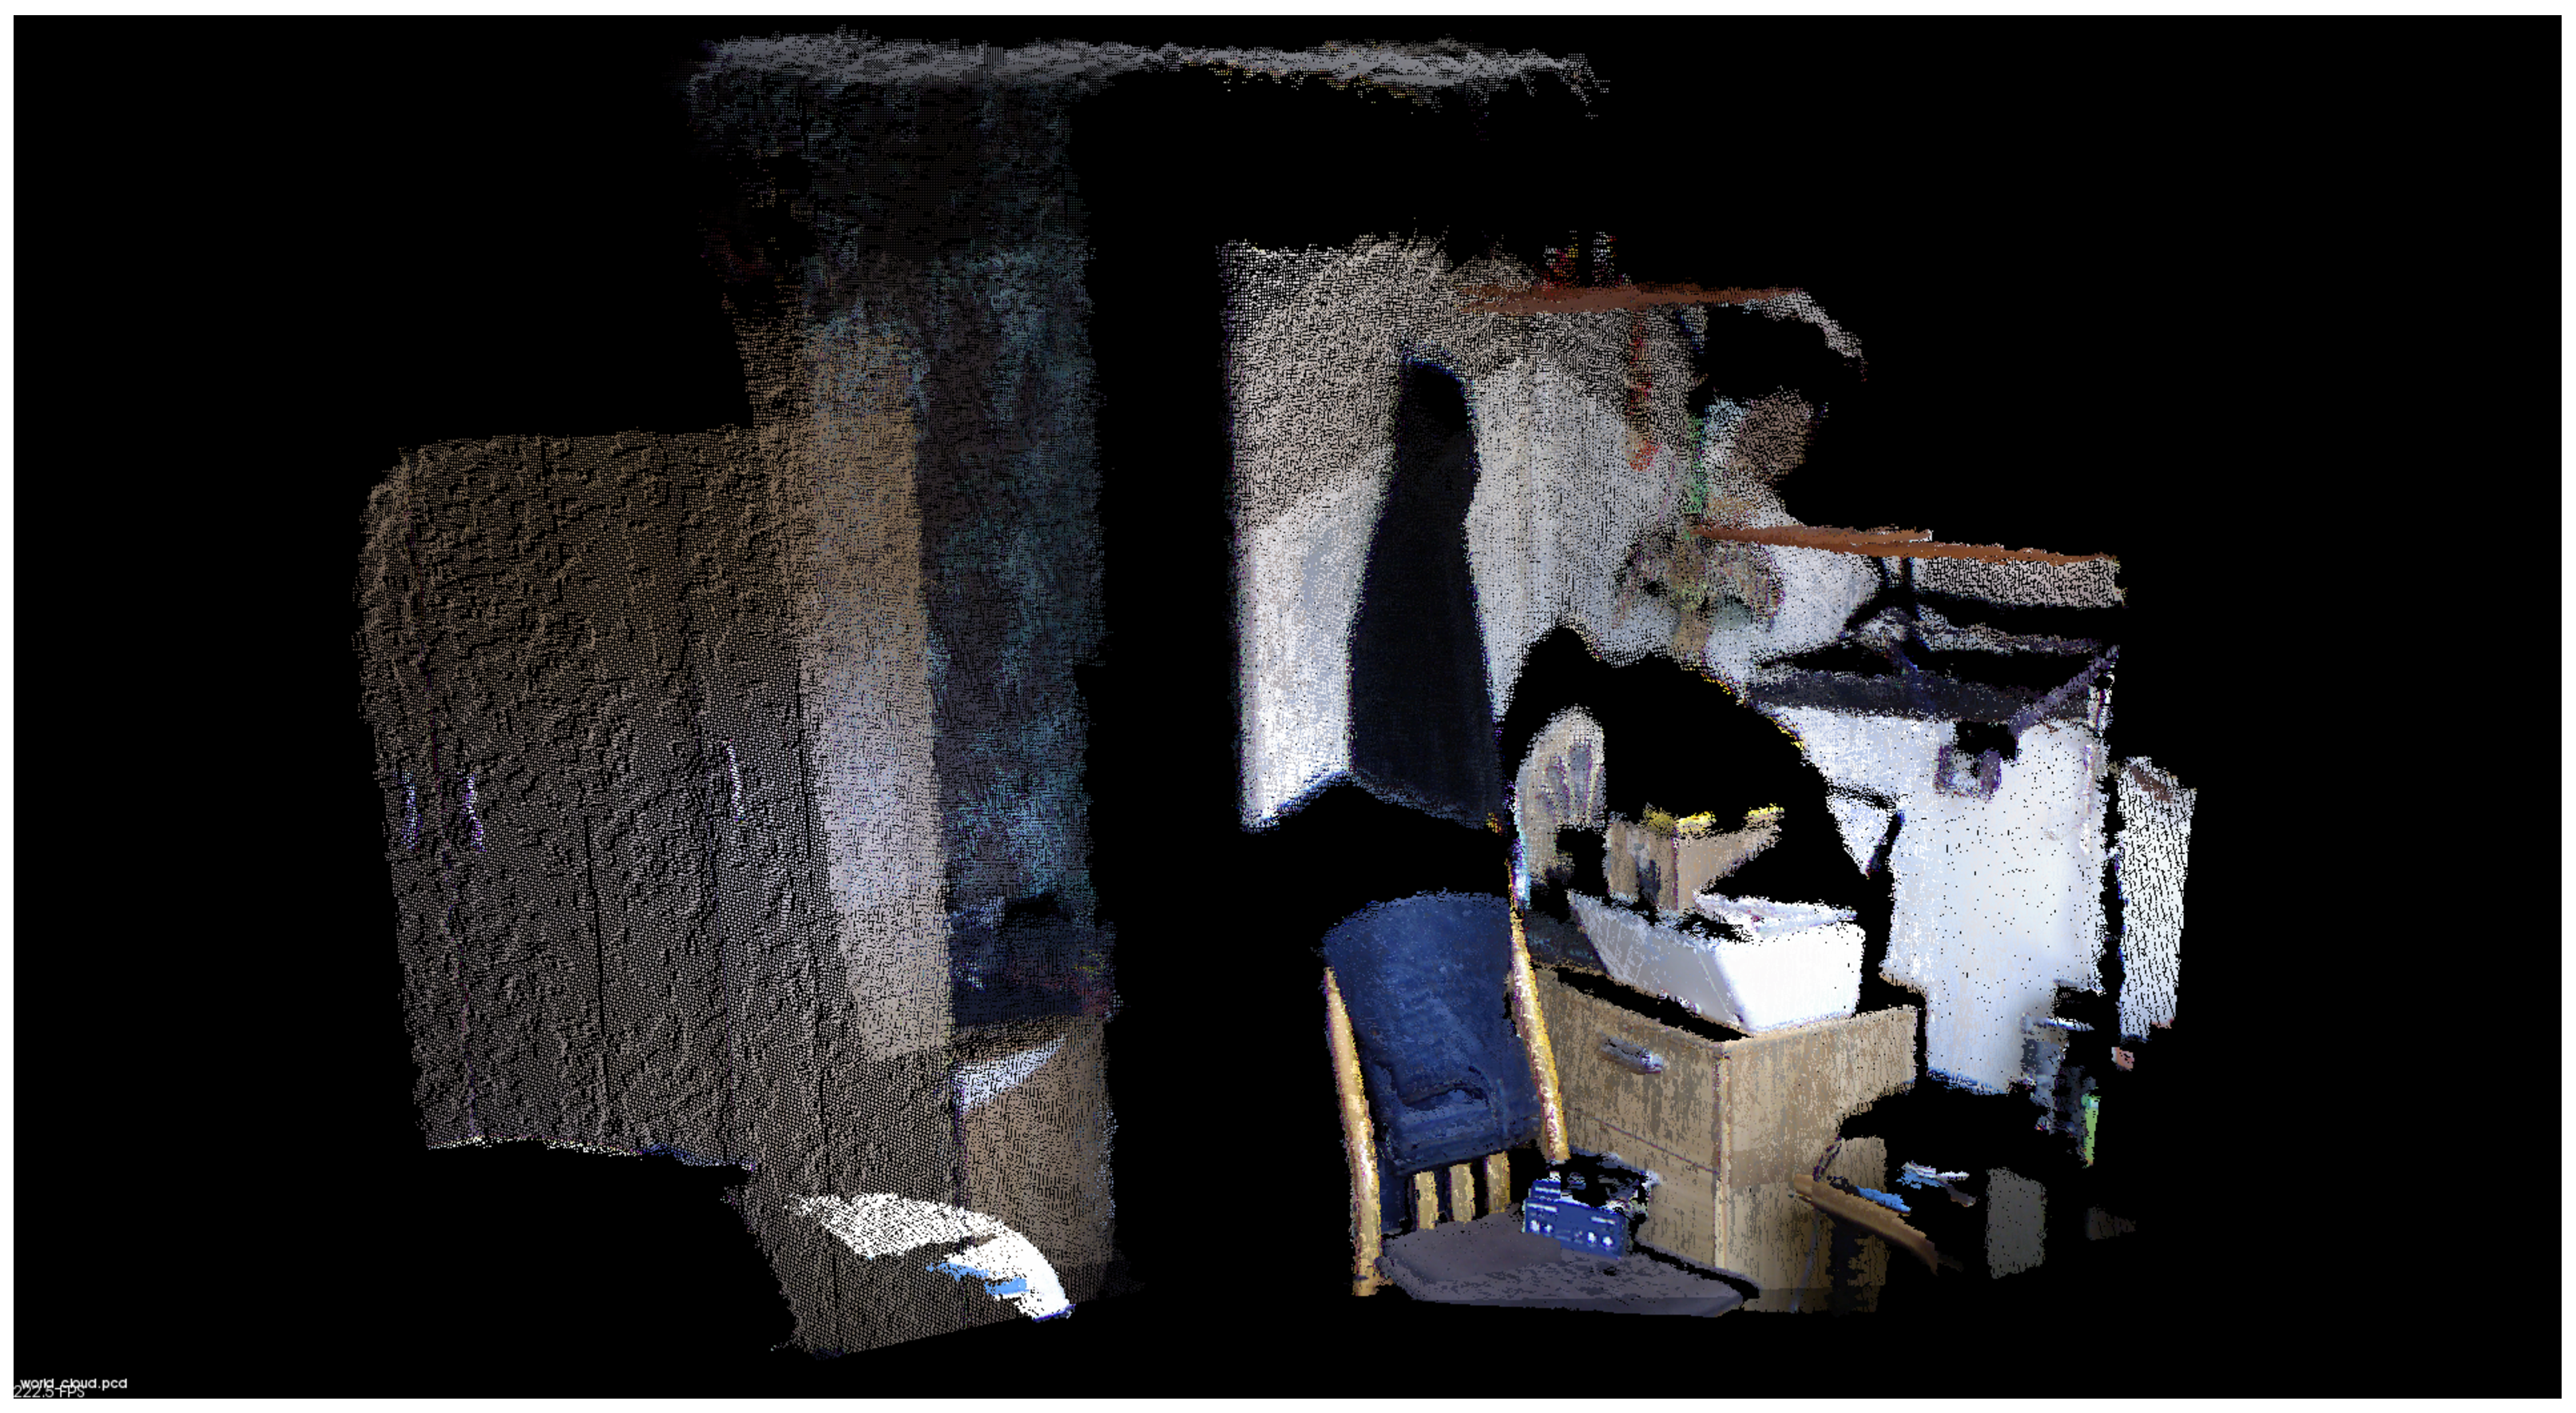
\includegraphics[width=0.7\textwidth]{graphics/room_1_world_ndt.eps}
  \caption{Room scan 1 IMU \& NDT registered cloud}
  \label{fig:room_1_ndt}
\end{figure}

This shows a registration that closely matches the results of the feature based
registration. There is very little noticeable misalignment and the sharp corners
of objects appear to align correctly.

Figure \ref{fig:room_2_transformed} shows the second room scan consisting of six
point clouds with nothing but the IMU obtain transformations applied.

\begin{figure}[h!]
  \centering
  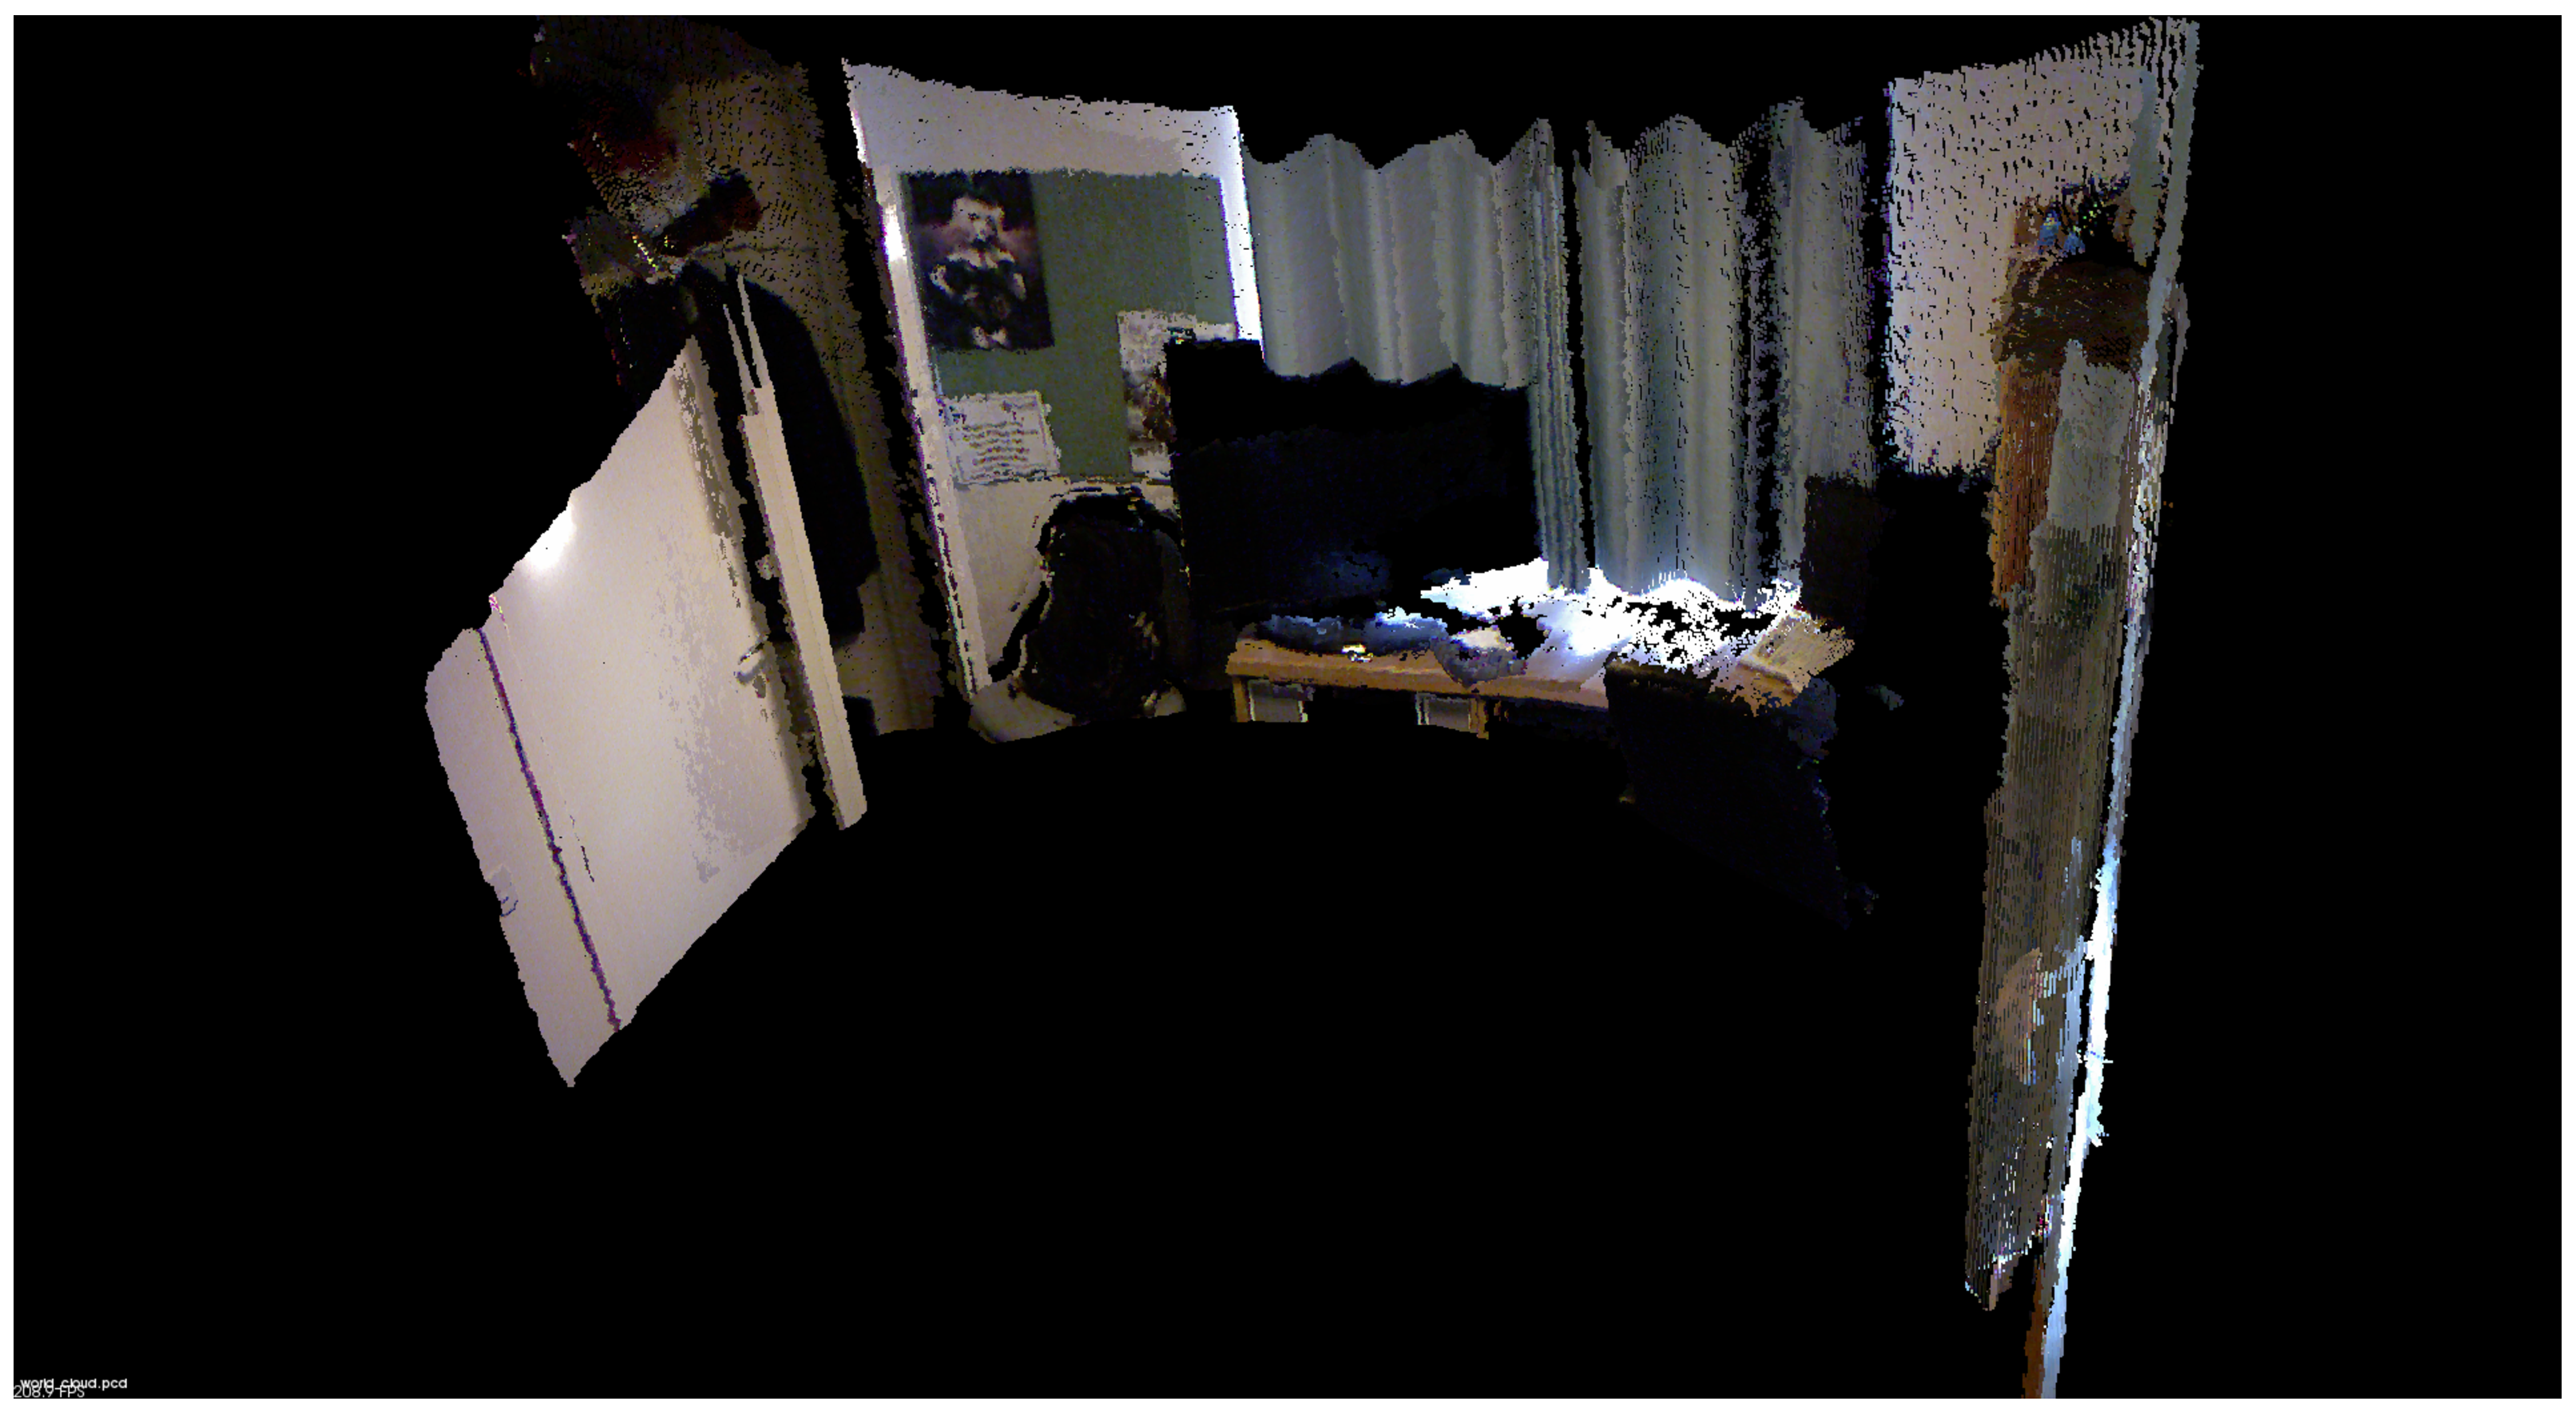
\includegraphics[width=0.7\textwidth]{graphics/room_2_transformed.eps}
  \caption{Room scan 2 transformed cloud}
  \label{fig:room_2_transformed}
\end{figure}

There are several obvious areas where IMU error has contributed to misalignment
of the captured point clouds. The most notable are the curtains in the centre of
the viewport and white door to the left.

Figure \ref{fig:room_2_icp} shows these point clouds registered using the ICP
based world registration workflow.

\begin{figure}[h!]
  \centering
  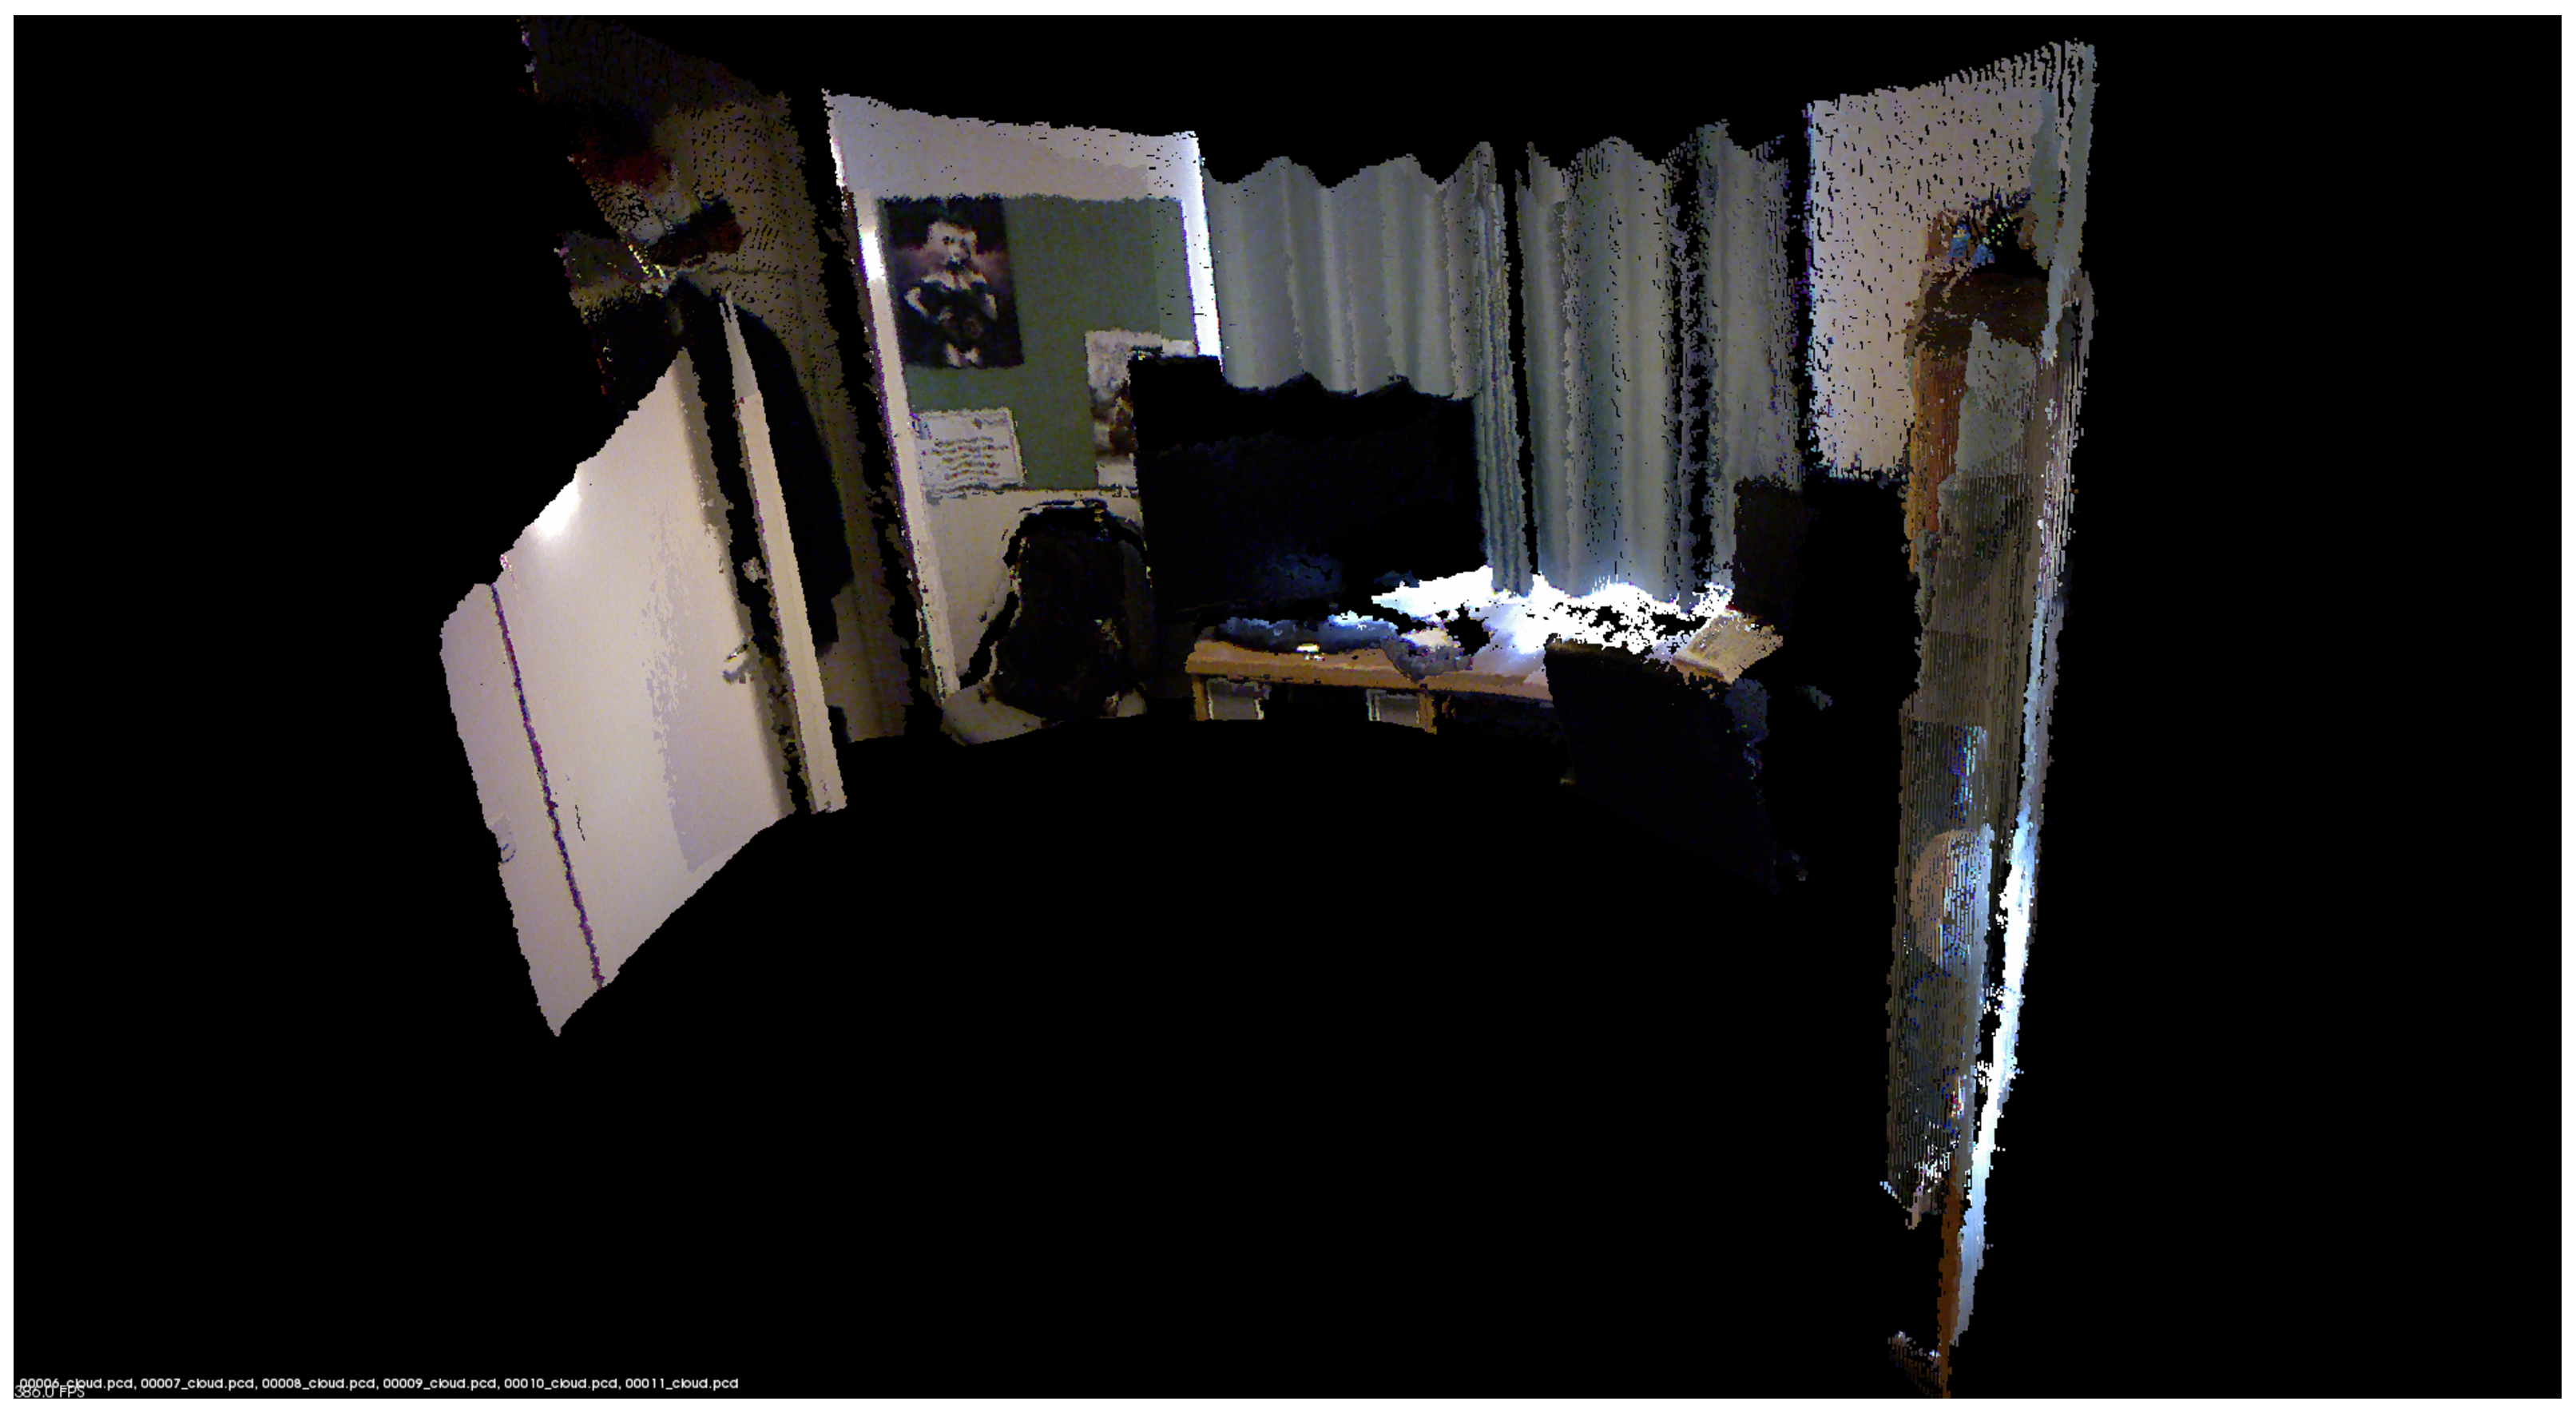
\includegraphics[width=0.7\textwidth]{graphics/room_2_world_icp.eps}
  \caption{Room scan 2 IMU \& ICP registered cloud}
  \label{fig:room_2_icp}
\end{figure}

This registration, whilst better then the IMU transformations alone, is not
ideal. The previously mentioned misalignments are still present, however the
alignment of the point clouds containing the door to the left have noticeably
improved.

\subsubsection{Short range desk scan}

Figure \ref{fig:desk_transformed} shows four point clouds from a scan of a desk
from approximately 1m away transformed by only IMU measurements.

Given the short distance between camera and subject error in the IMU measurement
contributes less of an alignment error, when error is measured as the Euclidean
distance between key points of the captured geometry.

\begin{figure}[h!]
  \centering
  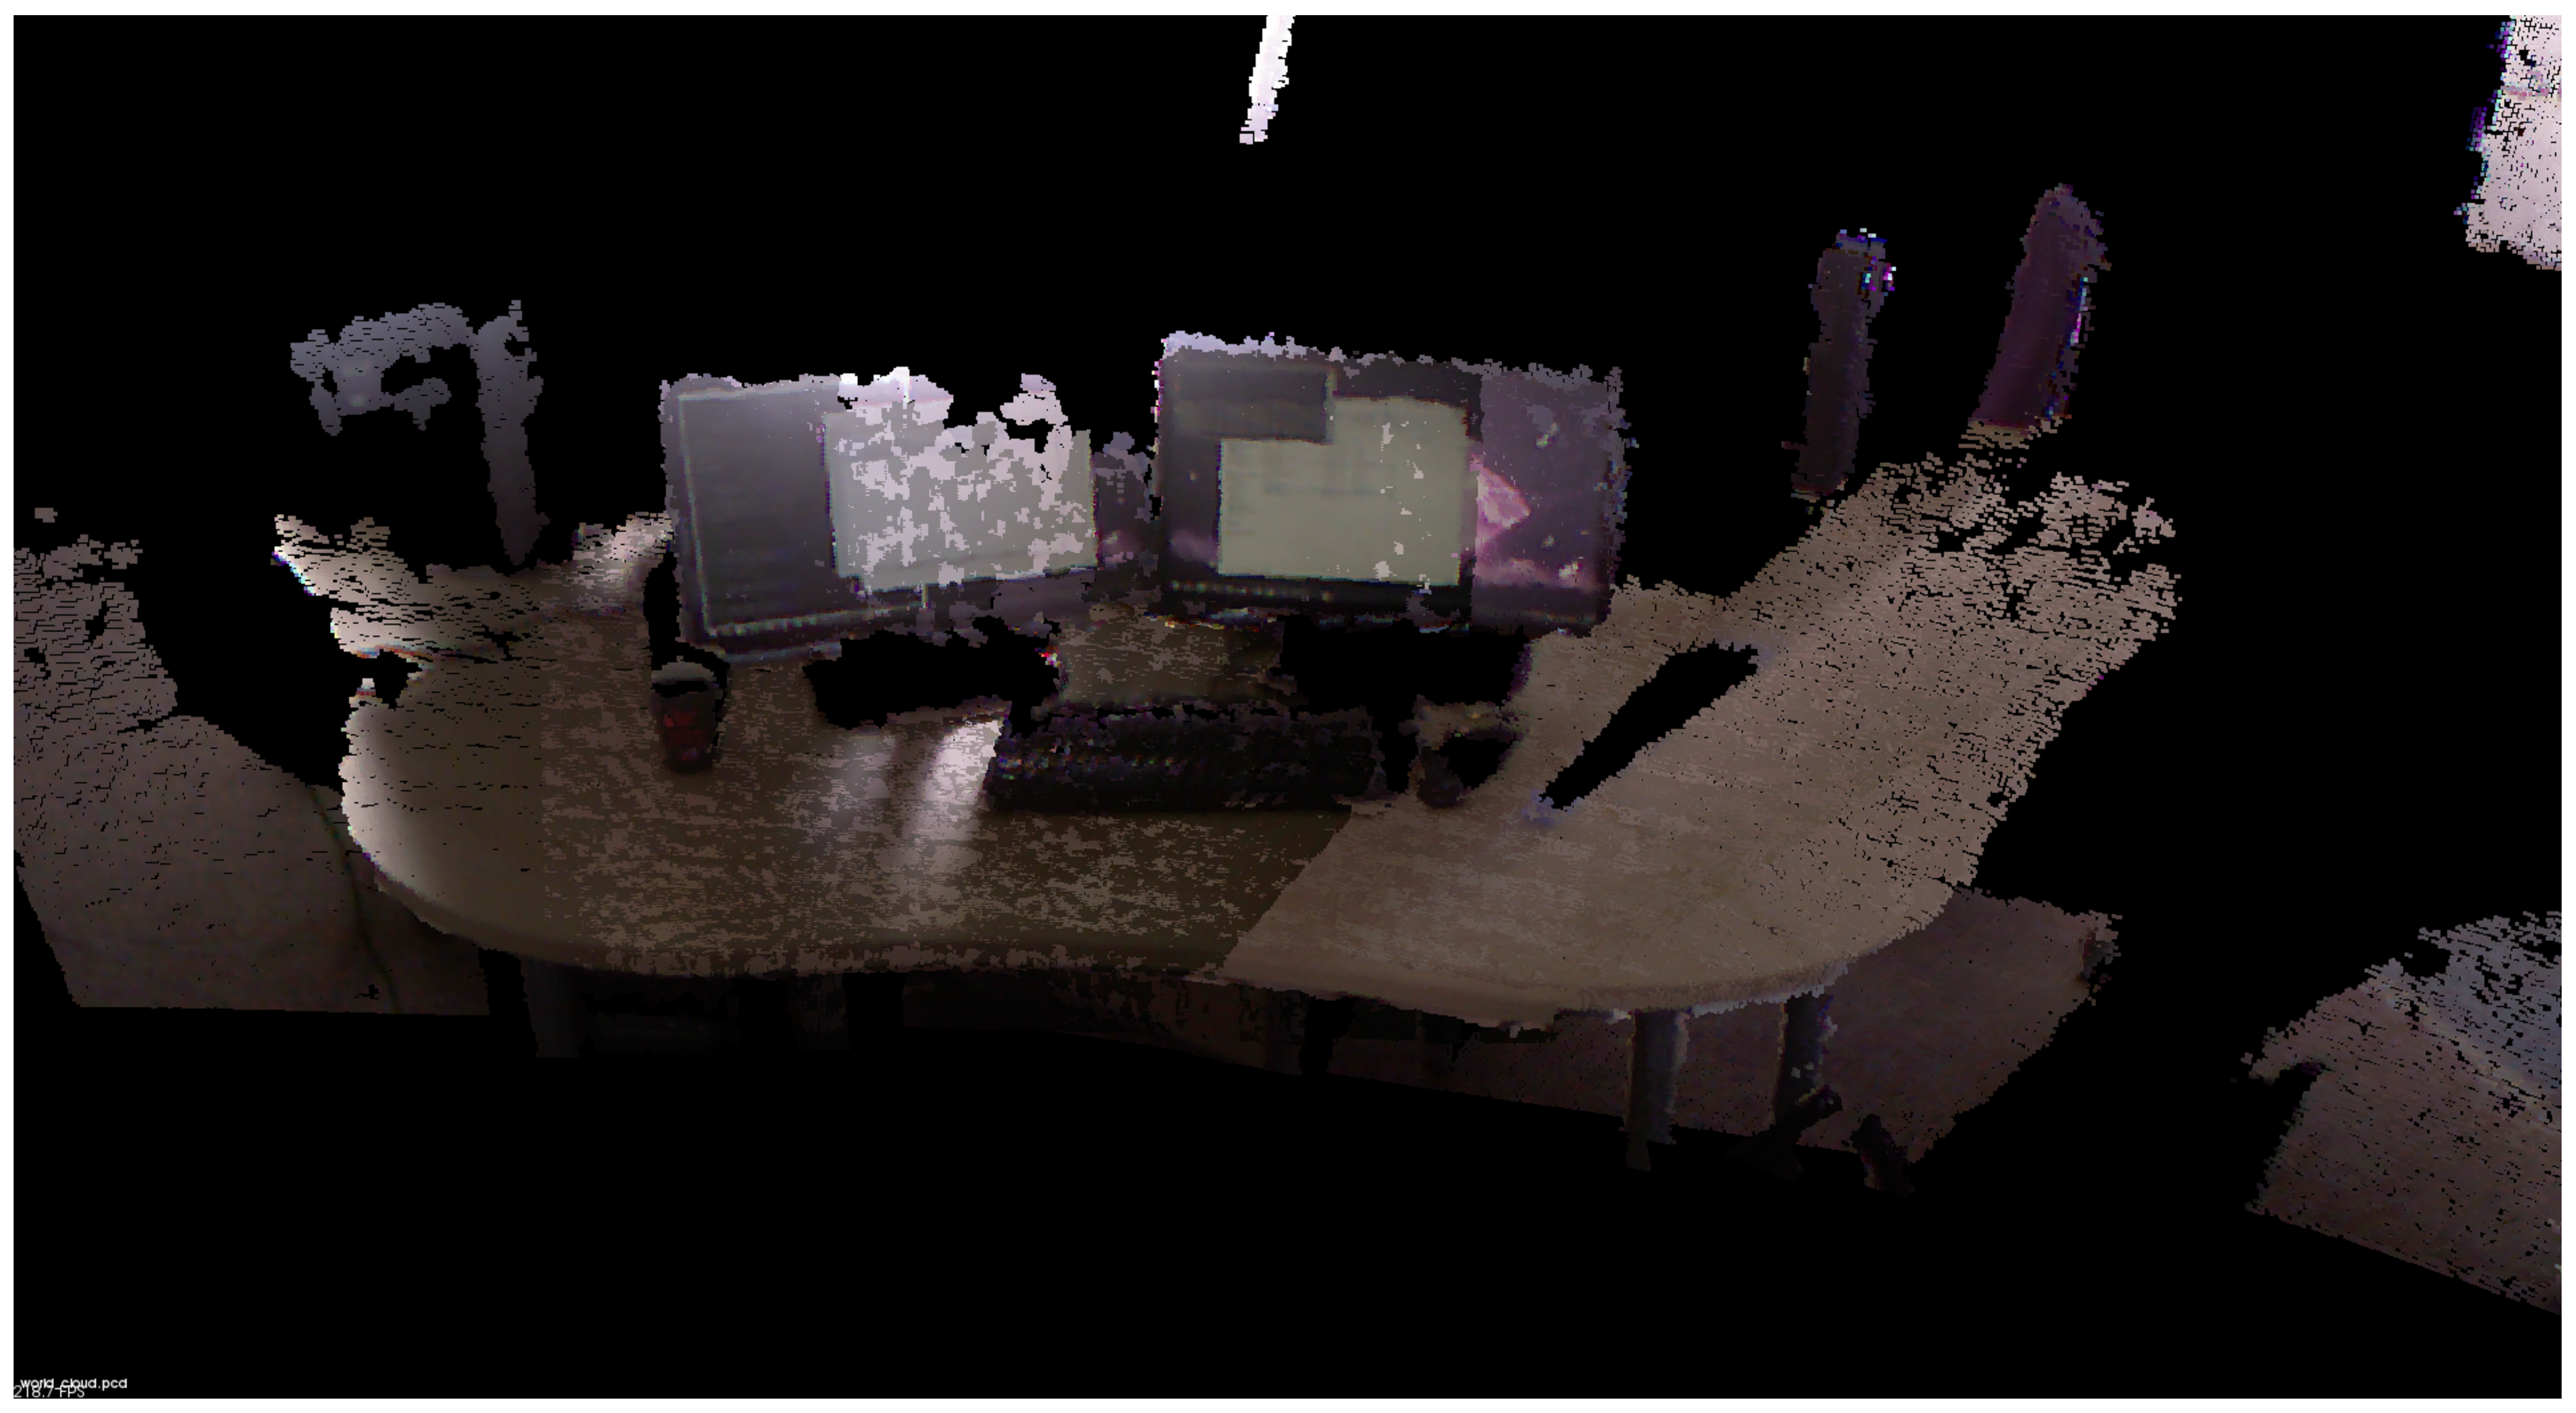
\includegraphics[width=0.7\textwidth]{graphics/desk_transformed.eps}
  \caption{Desk scan transformed cloud}
  \label{fig:desk_transformed}
\end{figure}

Such reduction in error can be seen in the transformed point clouds as there is
very little noticeable misalignment between adjacent clouds.

\begin{figure}[h!]
  \centering
  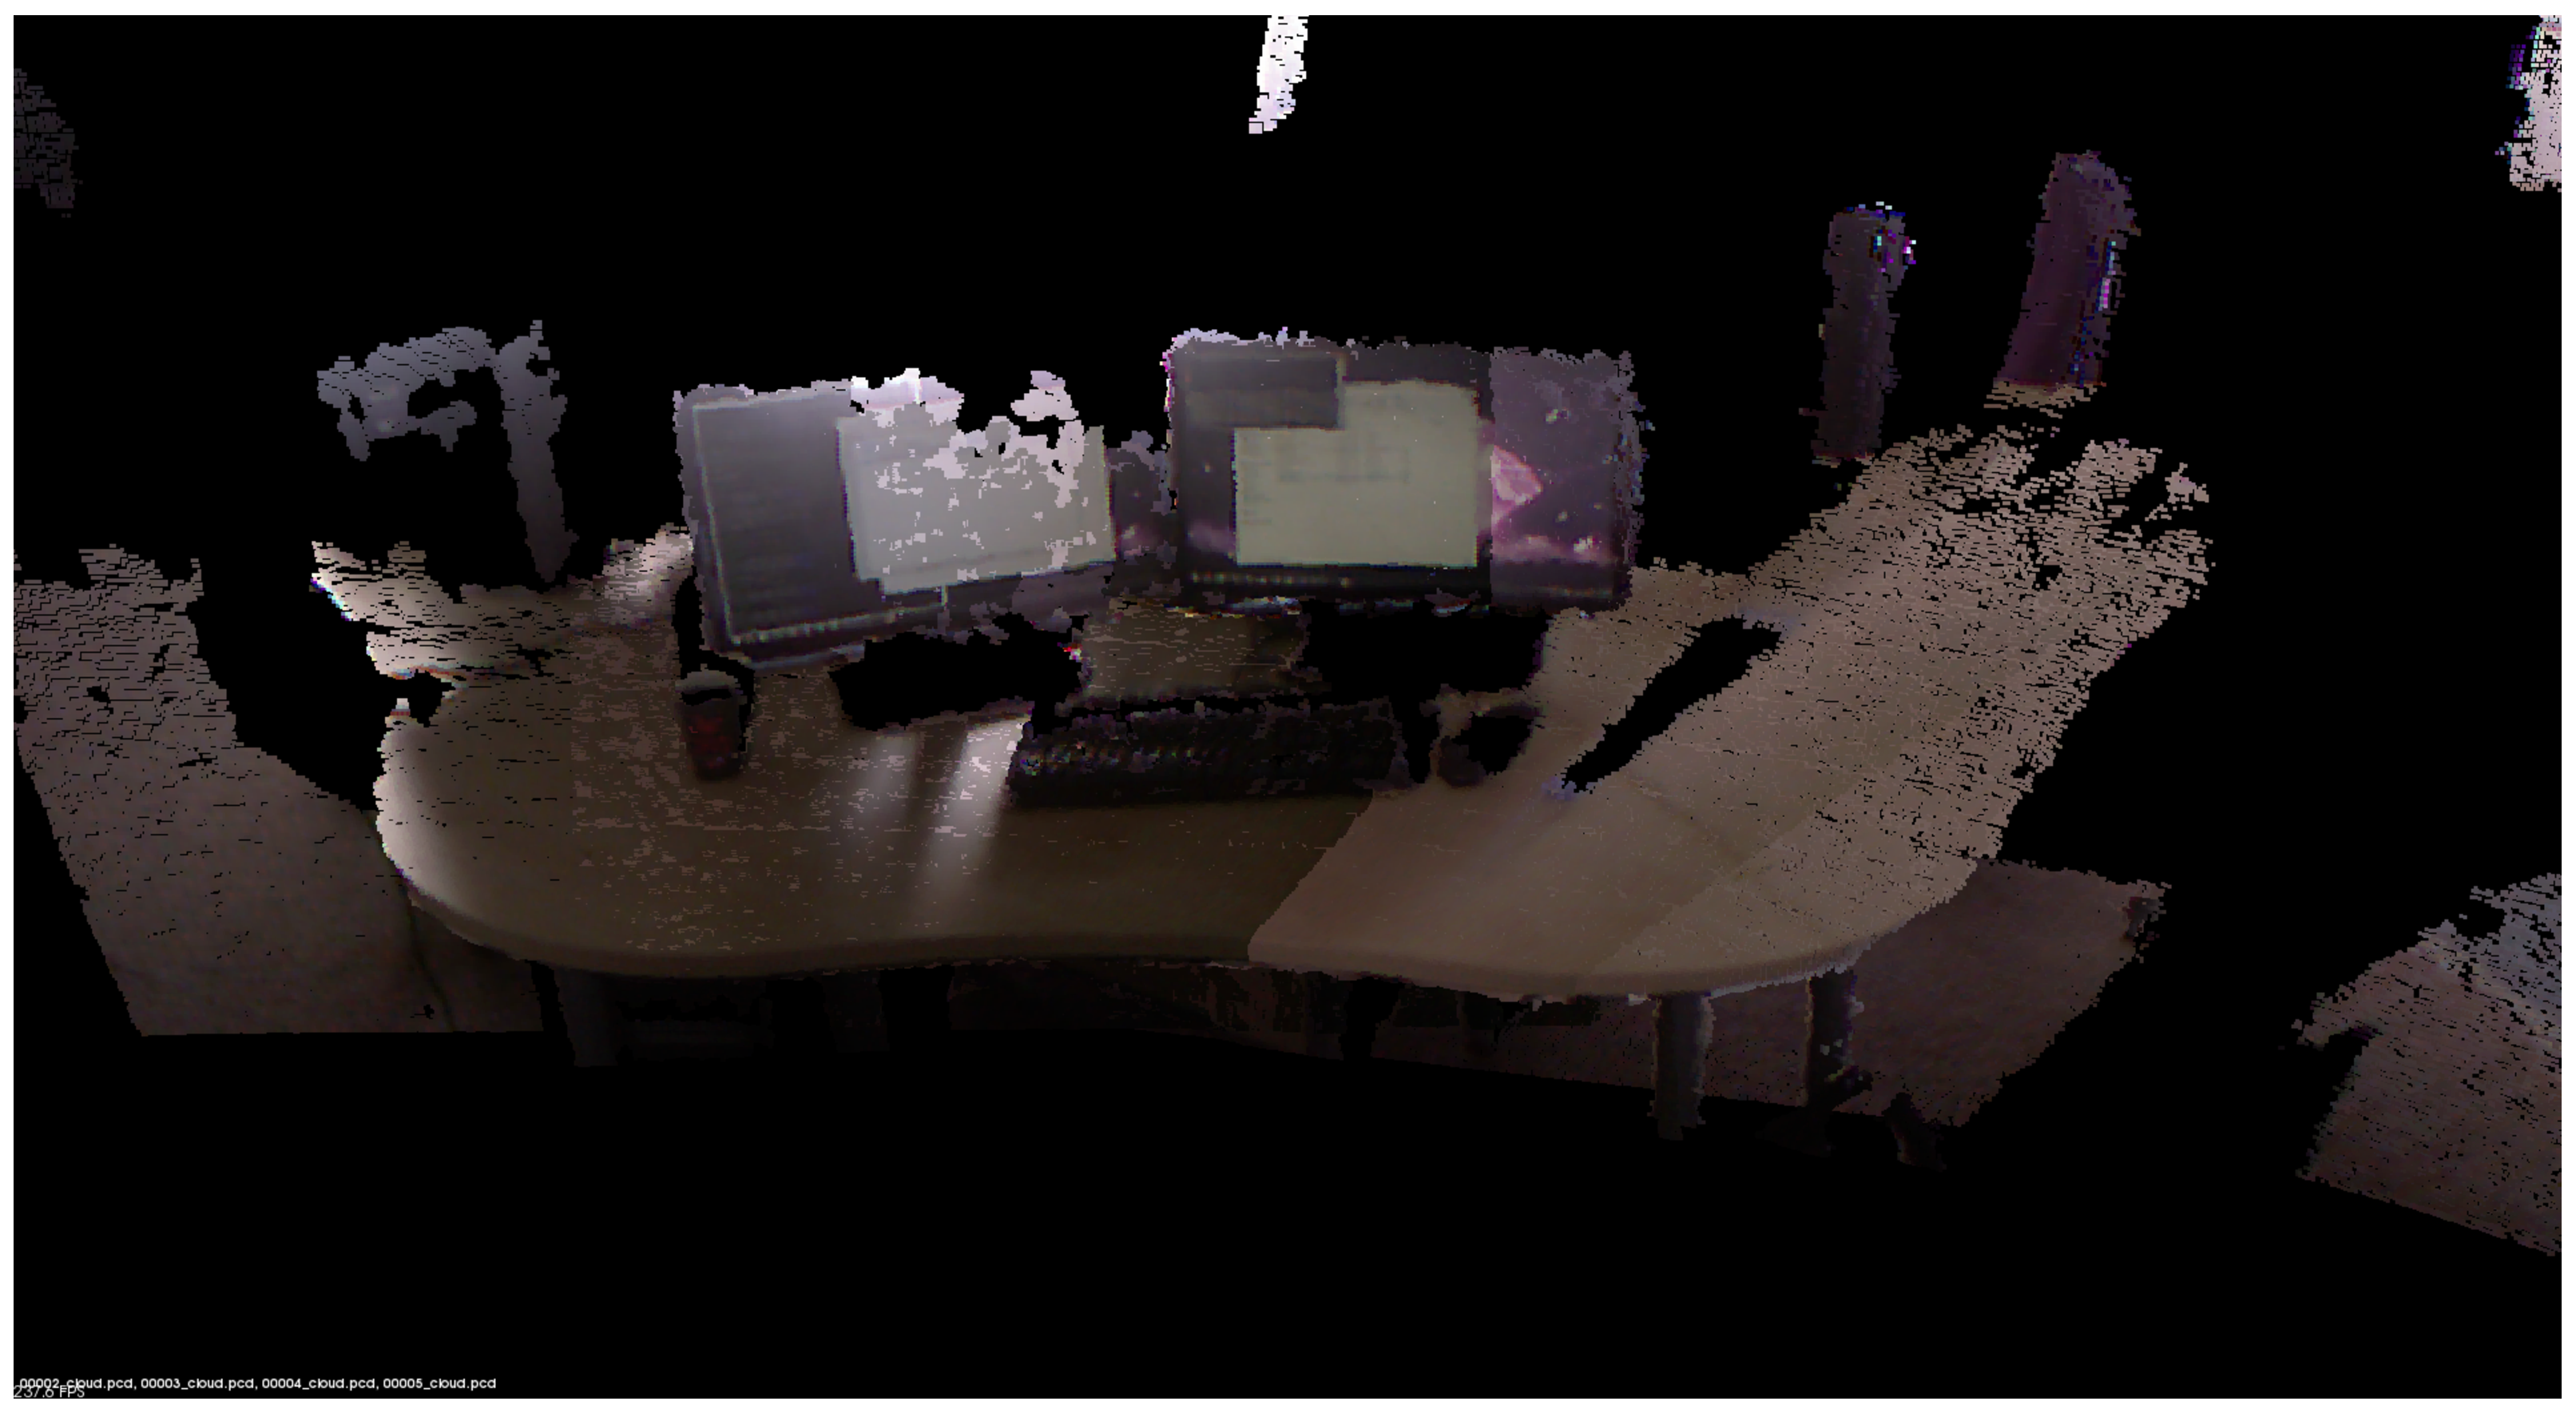
\includegraphics[width=0.7\textwidth]{graphics/desk_world_ndt.eps}
  \caption{Desk scan IMU \& NDT registered cloud}
  \label{fig:desk_ndt}
\end{figure}

The NDT based world alignment of these point clouds as shown in figure
\ref{fig:desk_ndt} shows only marginal improvement over the original IMU
transformations.

The front edge of the desk does appear to be smoother towards the right hand
side near the desk legs and there is reduced $z$-fighting is the rendering of
the point clouds, implying an overall improvement in the alignment of the desk
surface.

\subsection{IMU performance}

Given that the ability of IMU odometery to benefit the registration of point
clouds is highly dependant on the performance of the odometer itself, this will
be evaluated as a separate system.

This separation also allows a purely numerical evaluation to be carried out with
greater ease than when incorporated into the complete system.

The test setup consisted of the three implemented odometry systems being bolted
together in a stack as shown in the photo in figure \ref{fig:imu_test_setup},
this ensured that they remained aligned and all motion affected each IMU to the
greatest degree possible.

From top to bottom the stack consists of an Invensense MPU9150 breakout board,
an Omnibus F4 flight control board (running the STM32 odometer), a Motolab
Cyclone flight control board (running Betaflight acting as the "Vanilla MSP"
device) and a Teensy 3.2 (connected to the MPU9150 board, running the Teensy
odometer).

\begin{figure}[h!]
  \centering
  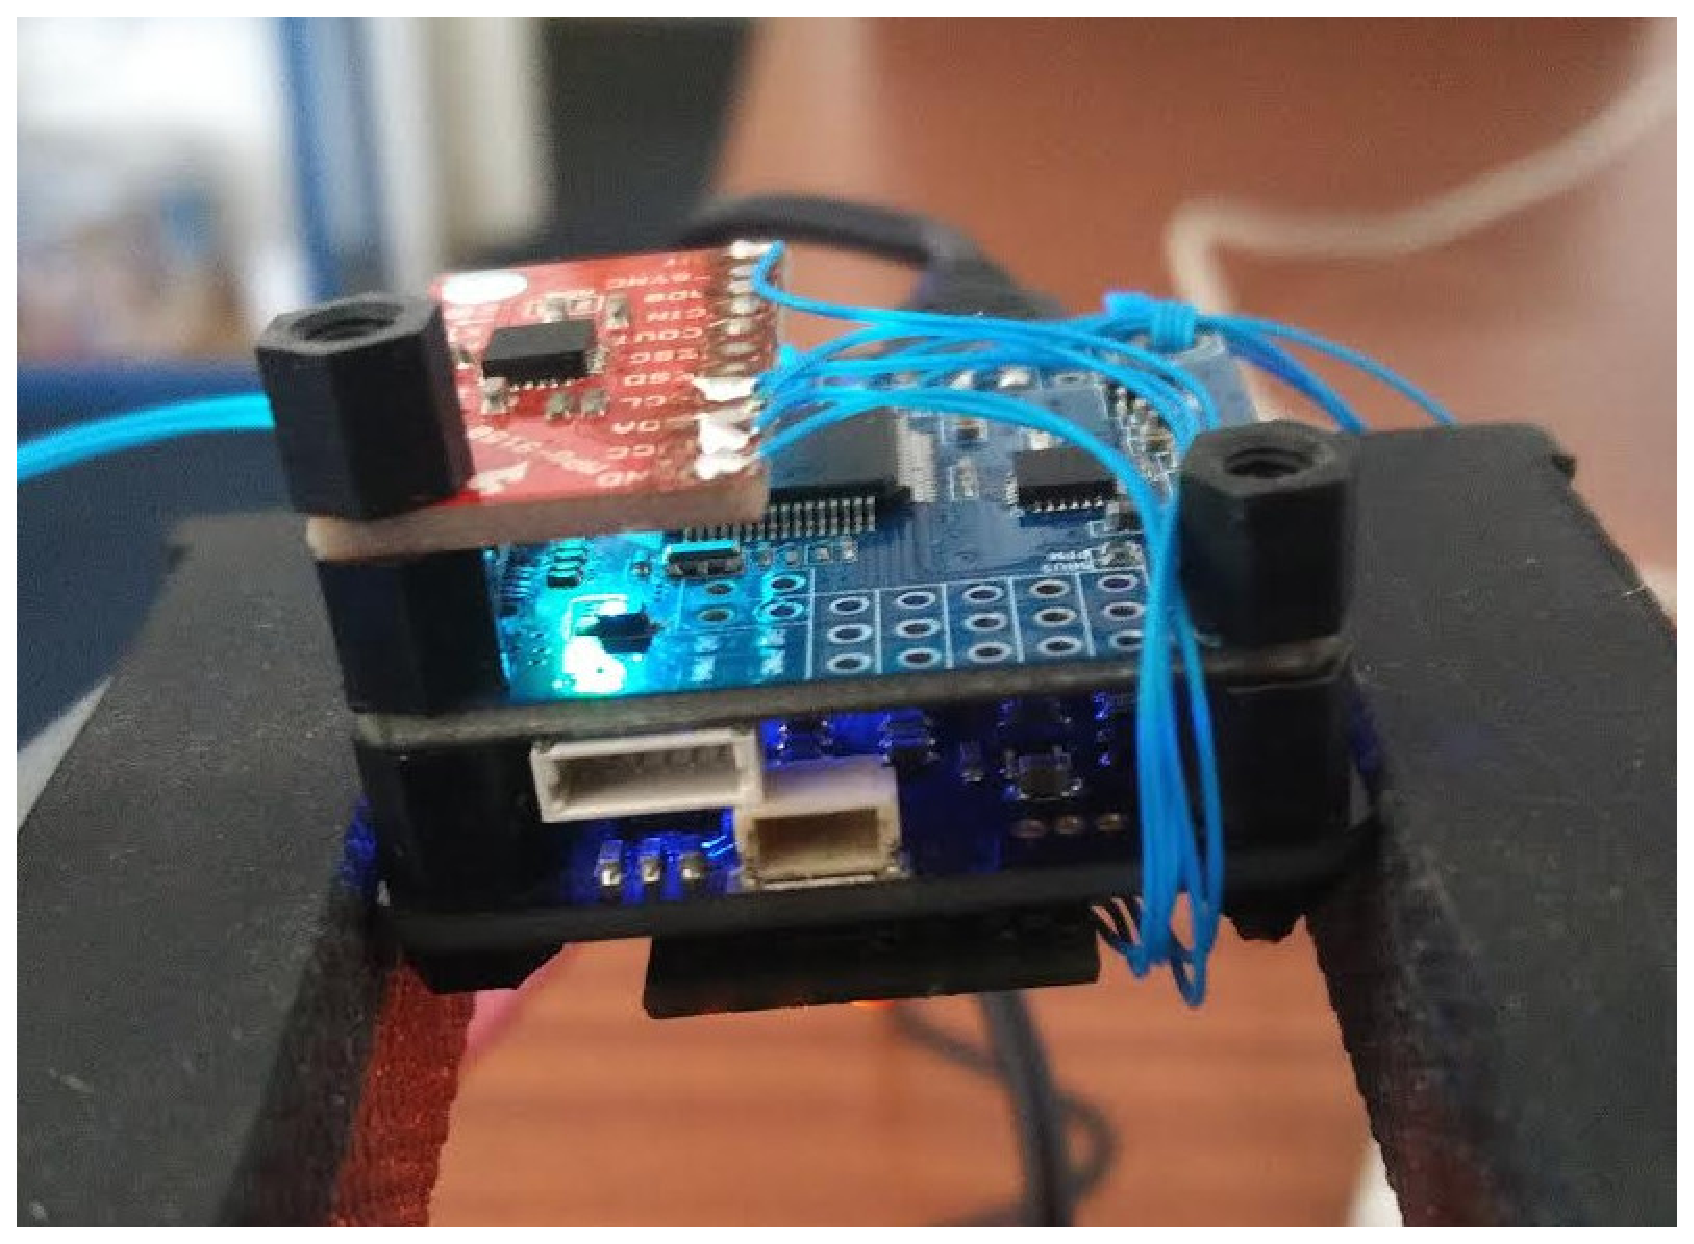
\includegraphics[width=0.5\textwidth]{graphics/imu_test_setup.eps}
  \caption{Odometer test setup}
  \label{fig:imu_test_setup}
\end{figure}

All units involving orientation are coefficients of a unit quaternion. All units
involving position are in metres, $m$; velocity is $ms^{-1}$ and acceleration is
$ms^{-2}$.

The X axis units in all results are sample number and can be seen as an
arbitrary measure of time. This sample number does not directly relate to the
IMU sample frequency.

In all tests involving position only the Teensy and STM32 based odometers took
part, this is due to the fact the "Vanilla MSP" odometer only supports
orientation tracking.

\subsubsection{Orientation stability}

The aim of this test is to ensure that the position reported by each IMU does
not drift whilst the device is stationary.

Error or drift in the orientation will add additional error into the initial
estimation used in the point cloud registration algorithms that will likely
result in longer execution times or lower quality registration.

In this test the devices were placed in a stationary position and the
calibration routines run. The reported orientation was then recorded (in
quaternion form) over a 15 minute period.

In the ideal case the reported orientation would not change over the length of
the test. Realistically some variation is expected as MEMS IMUs do suffer from
slight drift.

The results of this test are shown in figures
\ref{fig:15_min_orientation_stability_msp},
\ref{fig:15_min_orientation_stability_teensy} and
\ref{fig:15_min_orientation_stability_stm32} for the MSP, Teensy and STM32 based
implementations respectively.

\begin{figure}[h!]
  \centering
  \scalebox{0.7}{\input{data/15_min_orientation_stability_msp.tex}}
  \caption{MSP orientation stability (15 minutes)}
  \label{fig:15_min_orientation_stability_msp}
\end{figure}

The "Vanilla MSP" method gave relatively stable performance with a small amount
of drift around the vertical ("yaw") axis. This manifests itself in the steadily
changing Z and X components either side of the point at which the sign of the W
component changes.

There is a more significant drift in the Y component which is most likely due to
a systematic error as a similar effect can be seen in the tests of all other
odometers.

\begin{figure}[h!]
  \centering
  \scalebox{0.7}{\input{data/15_min_orientation_stability_teensy.tex}}
  \caption{Teensy orientation stability (15 minutes)}
  \label{fig:15_min_orientation_stability_teensy}
\end{figure}

The Teensy based IMU gave very stable performance with very little fluctuation
in the orientation components.

The only drift present is the systematic error that manifests itself in the Y
component of the orientation quaternion. Given that all IMUs were calibrated
after being assembled into the test stack with the "forward" directions facing
the same direction it can be assumed that the quaternion components are
equivalent across devices.

\begin{figure}[h!]
  \centering
  \scalebox{0.7}{\input{data/15_min_orientation_stability_stm32.tex}}
  \caption{STM32 orientation stability (15 minutes)}
  \label{fig:15_min_orientation_stability_stm32}
\end{figure}

The STM32 based IMU gave noticeably more drift that the Teensy IMU.

Given the issues seen on the other two IMUs no practical conclusions about the
performance can be derived form the Y element of the orientation quaternion.
However the drift on the X axis is unlikely to be from any environmental source
and is therefore indicative of IMU error.

As there is very little filtering on the raw values obtained from the MPU6000 in
this implementation it is possible that this drift is a result of noise from the
gyroscope being integrated by the orientation filter.

This could partly be corrected by altering the parameters of the filter to
include a greater corrective contribution from the accelerometer, however as the
accelerometer is a slower sensor this would add delay between angular velocity
reaching zero and the orientation stabilising. Although this is not inherently
an issue for orientation sensing, it may become a problem when the orientation
is used to transform the acceleration into the world frame.

\subsubsection{Orientation accuracy and error}

This test focuses on the accuracy of the orientation reported by each odometer.

In this test each device was set in a level position and the IMUs calibrated.
The test stack was then rotated between -45 and 45 degrees around the X
(pitch) and Y (roll) axes.

An IMU passes this test if the orientation reported by the device matches to an
acceptable degree of accuracy that which it was placed in.

The orientation in quaternion form was recorded using the
\texttt{IMUGrabberTest} program and converted to yaw/pitch/roll angles using
equation \ref{eq:quat_to_ypr}. This makes comparison between recorded result and
physical actuation of the sensor simpler.

\begin{equation}
  \left[
    \begin{array}{c}
      pitch\\
      yaw\\
      roll\\
    \end{array}
  \right]
  =
  \left[
    \begin{array}{c}
      arctan\left(\frac{2(wx+yz)}{1-2(x^{2}+y^{2}}\right)\\
      arcsin\left(2(wy-zx)\right)\\
      arctan\left(\frac{2(wz+xy)}{1-2(y^{2}-z^{2})}\right)\\
    \end{array}
  \right]
  \label{eq:quat_to_ypr}
\end{equation}

The results of this test are shown in figures \ref{fig:45_deg_movements_msp},
\ref{fig:45_deg_movements_teensy} and \ref{fig:45_deg_movements_stm32} for the
MSP, Teensy and STM32 based implementations respectively.

\begin{figure}[h!]
  \centering
  \scalebox{0.7}{\input{data/45_deg_movements_msp_ypr.tex}}
  \caption{MSP 45 degree movements}
  \label{fig:45_deg_movements_msp}
\end{figure}

The "Vanilla MSP" IMU performed well and returned an accurate representation of
the way it was moved.

\begin{figure}[h!]
  \centering
  \scalebox{0.7}{\input{data/45_deg_movements_teensy_ypr.tex}}
  \caption{Teensy 45 degree movements}
  \label{fig:45_deg_movements_teensy}
\end{figure}

The Teensy based IMU also performed well, however there is a significant offset
in the yaw angle.

This is most likely caused by noise during calibration or board misalignment.

\begin{figure}[h!]
  \centering
  \scalebox{0.7}{\input{data/45_deg_movements_stm32_ypr.tex}}
  \caption{STM32 45 degree movements}
  \label{fig:45_deg_movements_stm32}
\end{figure}

One thing that can be noticed about the results of the STM32 based IMU is that
the reported deflection in each direction is reliably 1-2 degrees lower than the
other two implementations.

The most likely reason for this is insufficient weighting of the accelerometer
in the orientation filter. A greater corrective contribution from an absolute
device should correct for offset errors introduced.

All three implementations performed well in this test with no significant
issues.

\subsubsection{Stationary error whilst level}

The first test of the positioning part of the odometer was to ensure that when
the sensor is level and stationary there was no motion being reported.

In this test the test IMUs were placed into a stationary position, the
calibration procedures run and the integrators for velocity and position reset.
The odometers were then left for 1 minute and the acceleration, velocity and
displacement on the X and Y axis recorded.

An IMU passes this test if for the duration of the test the acceleration in all
axis remains zero.

The results for the Teensy and STM32 based odometers are shown in figures
\ref{fig:teensy_stationary_level_error} and
\ref{fig:stm32_stationary_level_error} respectively.

\begin{figure}[h!]
  \centering
  \scalebox{0.7}{\input{data/teensy_level_disp.tex}}
  \caption{Teensy stationary error whilst level}
  \label{fig:teensy_stationary_level_error}
\end{figure}

With the Teensy based IMU there is frequent noise that manifests as large spikes
on the X and Y acceleration which in turn causes a gradually more diverging
velocity and displacement.

The specific cause of this was not clear as when sampling raw values from the
accelerometer such noise spikes were not found, therefore the source of the
issue is likely to either be gyroscope noise which in turn effects the gravity
vector or in the implementation of the low pass filter used to smooth
world acceleration samples.

\begin{figure}[h!]
  \centering
  \scalebox{0.7}{\input{data/stm32_level_disp.tex}}
  \caption{STM32 stationary error whilst level}
  \label{fig:stm32_stationary_level_error}
\end{figure}

The STM32 based odometer gave reasonable performance in that the amount of drift
due to a non zero acceleration was minimal, however there was sufficient noise
in the raw accelerometer data to prevent a consistently low reading which would
fall below the acceleration threshold and in turn eventually trigger the end of
motion and reset the velocity to zero.

\subsubsection{Stationary error whilst in angular motion}
\label{sec:stat_error_45deg}

This test involved verifying that when the IMU is rotated whilst kept linearly
stationary there would be no linear acceleration or change in velocity and
displacement recorded by the odometer.

In this test the IMUs were placed in a level position, calibrated and their
velocities and displacements reset. They were then rotated 45 degrees clockwise
around the X axis.

An IMU passes this test if the acceleration along the X and Y axis remains zero
whilst the device is under angular rotation.

The results for the Teensy and STM32 based odometers are shown in figures
\ref{fig:teensy_stationary_45deg_error} and
\ref{fig:stm32_stationary_45deg_error} respectively.

\begin{figure}[h!]
  \centering
  \scalebox{0.7}{\input{data/teensy_45deg_disp.tex}}
  \caption{Teensy stationary error whilst at 45 degrees}
  \label{fig:teensy_stationary_45deg_error}
\end{figure}

\begin{figure}[h!]
  \centering
  \scalebox{0.7}{\input{data/stm32_45deg_disp.tex}}
  \caption{STM32 stationary error whilst at 45 degrees}
  \label{fig:stm32_stationary_45deg_error}
\end{figure}

Both the Teensy bad STM32 based odometers displayed similar characteristics in
this test, in that neither correctly compensated for the orientation of the IMU
when calculating the acceleration in the world frame.

The spike in displacement on the STM32 based odometer is due to an
implementation error that manifests when the integrators for velocity and
position are reset whilst there is non zero acceleration on the IMU. In this
case the non zero acceleration was erroneous acceleration from the board not
being perfectly level.

\subsubsection{Motion error whilst level}

This test validated the ability of the IMU odometer to correctly report
displacement when it is moved in a single axis whilst being kept level.

In this test the IMUs were placed stationary, calibrated and their velocities
and displacements reset. They were them moved 0.9m along their Y axis, then 0.9m
in the opposite direction along the Y axis.

An IMU passes this test if the IMU reports a displacement of 0.9m after the
first motion and a displacement of 0m after the second motion.

The results for the Teensy and STM32 based odometers are shown in figures
\ref{fig:teensy_90cm_move} and \ref{fig:stm32_90cm_move} respectively.

\begin{figure}[h!]
  \centering
  \scalebox{0.7}{\input{data/teensy_90cm_move.tex}}
  \caption{Teensy 0.9m displacement whilst level}
  \label{fig:teensy_90cm_move}
\end{figure}

The Teensy based odometer recorded acceleration and velocity changes in the
correct direction for each move, however this produced inconsistent velocities
due to the large difference in magnitude despite the IMU being accelerated at
the same rate in both moves.

A possible cause of this is linked to the stability at an angle test carried out
in section \ref{sec:stat_error_45deg}, if the device was not perfectly level
during the second move then a certain contribution to this acceleration could be
error.

The odometer also failed to detect an end of motion state after each move was
complete and the device was relatively stationary.

Much of the issues with the Teensy implementation appear to be related to the
IMU missing data due to a too low sample frequency, however given the choice of
inter device communication and the use of on chip filtering and processing which
both limit the sampling frequency and add delay into the signal chain, this
implementation has a limited suitability for this application.

\begin{figure}[h!]
  \centering
  \scalebox{0.7}{\input{data/stm32_90cm_move.tex}}
  \caption{STM32 0.9m displacement whilst level}
  \label{fig:stm32_90cm_move}
\end{figure}

The STM32 based odometer performed significantly better than the Teensy. In each
move it reported a displacement in the correct direction of approximately the
correct magnitude.

The most significant issue was that the velocity often returned to zero before
the motion was complete, this led to velocity in the opposite direction being
reported at the end of the move which led to an offset from the correct
displacement.

A possible cause of this is lack of filtering on the raw accelerometer data, in
order to sample the IMU at the full 8kHz the digital low pass filtering in the
IMU was disabled and the only filtering in the odometry implementation was a
rudimentary low pass filter implemented as a window average.

Another possible issue could be the motion end condition being activated too
early, this would explain the sharp drop in velocity after the initial spike in
acceleration at the start and end of a move.

\section{Conclusion}

In general IMU odometery does provide several benefits over feature based
transformation estimation for registration of pairs of point clouds, however
given the measurement error of the implemented odometers can struggle to
provide an estimate of equal quality to that of feature based estimation.

An unforeseen advantage of an initial estimate taken from IMU data is that the
number of parameters that must be tuned to the environment is greatly reduced.
This does contribute to the goal of a workflow that is robust in a range of
different environments, however optimisation of the fine registration parameters
is typically still required to obtain the best results.

The quality of the initial estimate from IMU data does allow a reasonable
registration, however there is sufficient error present such that the fine
alignment methods typically do not converge on the optimal transformation
between point clouds. This error becomes more visible in the final registration
as the target gets further away from the camera.

\subsection{Further Work}

There are several possible improvements on the work carried out in this project
that would likely yield higher quality results. This section describes several
such improvements and what benefits they offer over what has been implemented in
this project.

\subsubsection{Hybrid incremental-world registration methods}
\label{sec:further_work_hybrid_registration}

It would be possible to overcome the issues of both incremental and world
registration methods using a hybrid of the two in which the world method is used
for small subsections of the world which are then registered incrementally.

This would limit the size of the world cloud that would be required to be kept
in memory whilst retaining the ability to move the camera view to arbitrary
positions.

\subsubsection{Automated 360 degree scanning}

An alternative method for capturing large environments could be to use a system
that automatically orients the camera to a given pitch and yaw angle which then
allows a 360 degree "bubble" scan to be performed automatically.

Several of these scans could then be aligned using a feature based approach,
possibly using positional information as an approximate initial transformation
if it is available.

Such a system has the advantage of removing the need to depend on accurate IMU
measurements, assuming that the positioning system had little error.

\subsubsection{Odometry data fusion}

Performing additional data fusion from other position/displacement providers on
the odometer device could be a valuable step in improving its positional
performance.

An obvious example could be to combine GPS positional data to correct for drift
in the displacement provided by the accelerometer. This would help towards
compensating for orientation error contributing to false acceleration in the
plane perpendicular to the gravity vector.

Another advantage of this would be obtaining an absolute position. This would be
most beneficial when performing multiple scans over a large area, for instance
scanning several buildings within a city.

Several MEMS IMUs could also be used to reduce error in gyroscope and
accelerometer measurements.

\subsubsection{Improved IMU filtering}

The tests of the IMU odometer alone show that in some cases the level of
filtering of the raw IMU data is not sufficient for the level of noise present
in the system.

In order to preserve the high sample rate but still benefit from filtered data
at least a configurable low pass filter should be implemented as the first part
of the signal chain after acquisition.

One possible implementation could be the finite impulse response filters
published by Mike Perkins at CardinalPeak \cite{perkins_fir_filters}.

\printbibliography

\appendix

\section{Class diagrams}

\begin{figure}[h!]
  \centering
  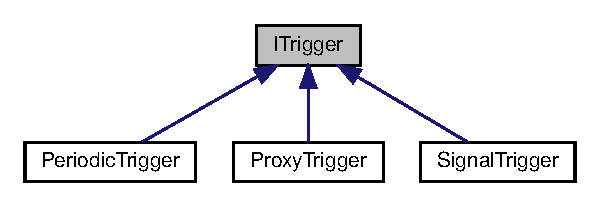
\includegraphics[width=0.5\textwidth]{graphics/triggers_class_diag.eps}
  \caption{Triggers UML diagram}
  \label{fig:framework_triggers}
\end{figure}

\begin{figure}[h!]
  \centering
  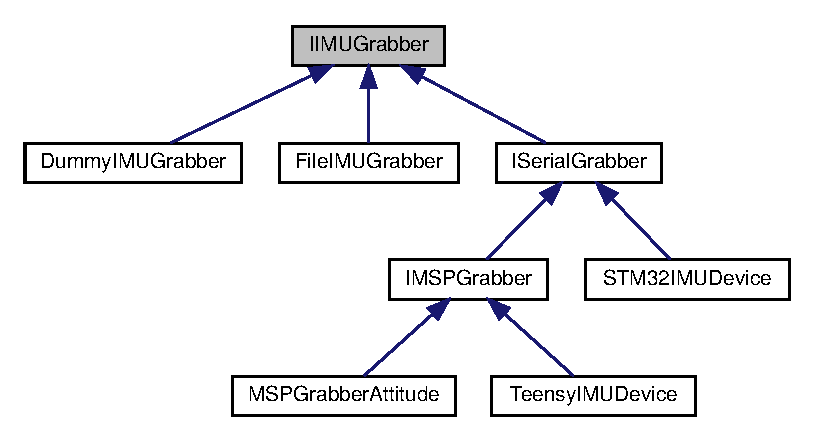
\includegraphics[width=0.6\textwidth]{graphics/imu_class_diag.eps}
  \caption{IMU drivers UML diagram}
  \label{fig:framework_imu}
\end{figure}

\begin{figure}[h!]
  \centering
  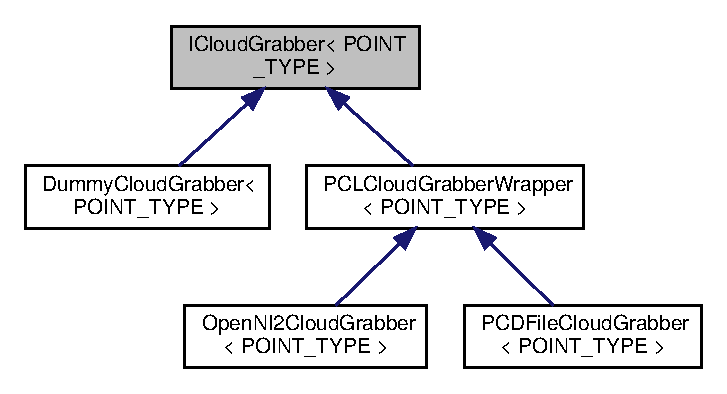
\includegraphics[width=0.5\textwidth]{graphics/cloudcapture_class_diag.eps}
  \caption{Point cloud capture UML diagram}
  \label{fig:framework_cloudcapture}
\end{figure}

\begin{figure}[h!]
  \centering
  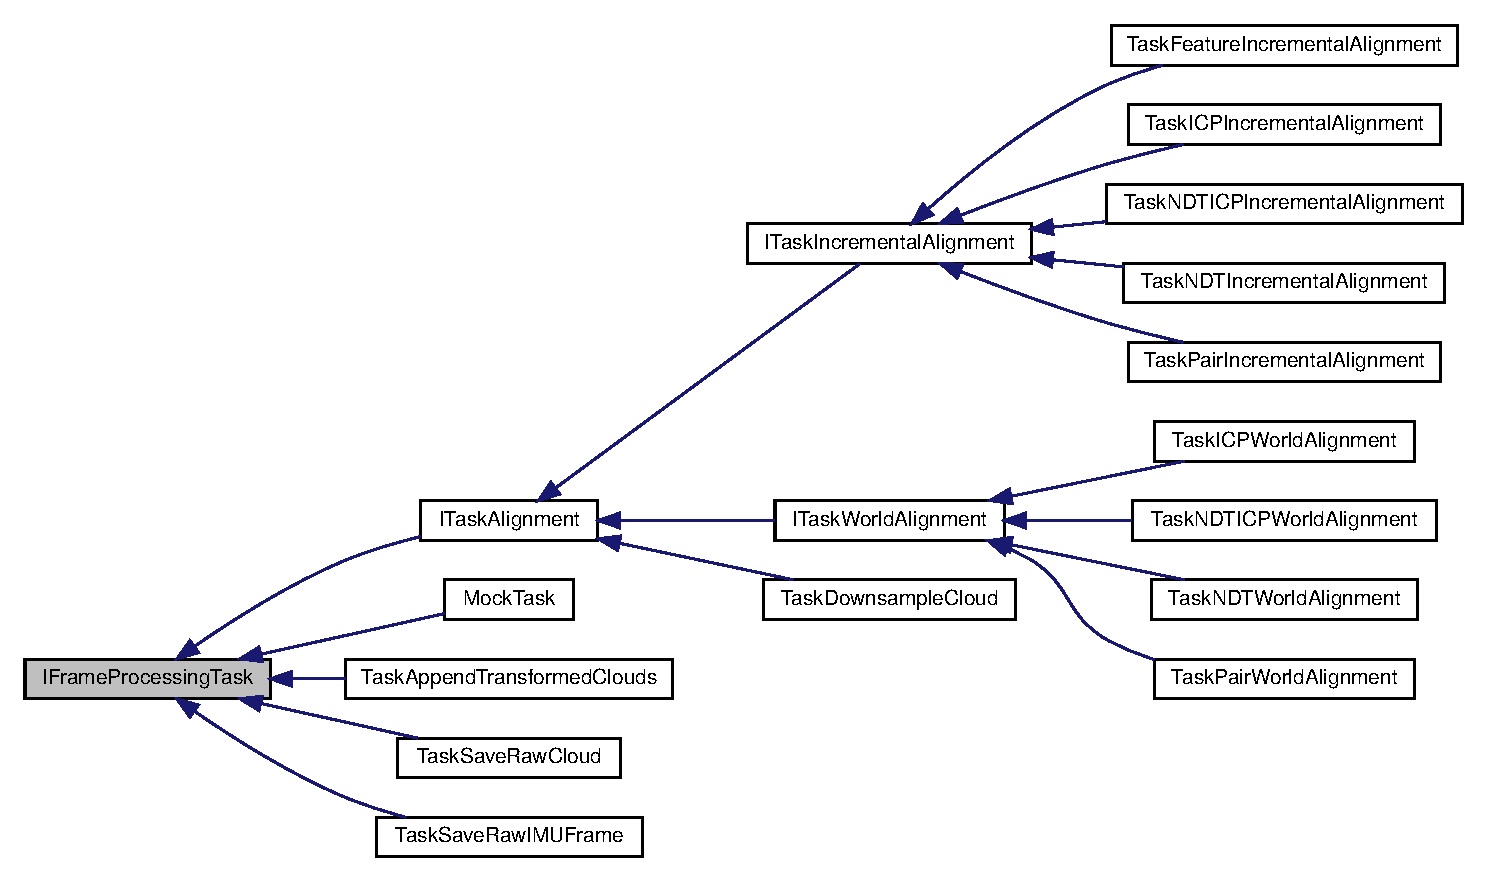
\includegraphics[width=\textwidth]{graphics/processing_class_diag.eps}
  \caption{Processing UML diagram}
  \label{fig:framework_processing}
\end{figure}

\end{document}
